\documentclass[conference]{IEEEtran}
\IEEEoverridecommandlockouts
\usepackage{cite}
\usepackage{amsmath,amssymb,amsfonts}
\usepackage{graphicx}
\usepackage{textcomp}
\usepackage{xcolor}
\usepackage{booktabs}
\usepackage{multirow}
\usepackage{placeins}
\usepackage{enumitem}
\usepackage{hyperref}
\usepackage{subfig}
\hypersetup{hidelinks}
\usepackage{tikz}
\usetikzlibrary{arrows.meta,positioning,calc}

\newcommand{\wasm}{\textsc{wasm}}
\newcommand{\ms}{\,ms}

% Architecture figure colors
\definecolor{hwblue}{RGB}{180,205,240}
\definecolor{osbrown}{RGB}{255,200,100}
\definecolor{wgreen}{RGB}{144,220,144}
\definecolor{cpurple}{RGB}{210,185,235}
\definecolor{cblue}{RGB}{150,195,235}
\definecolor{yorange}{RGB}{220,155,130}
\definecolor{gpink}{RGB}{255,200,200}

\begin{document}

\title{Web-Based Edge Computing for Optical Mark Recognition:\\
A Cross-Platform Performance Benchmark}

\author{%
\IEEEauthorblockN{Huy Kien Phan}
\IEEEauthorblockA{\texttt{huykien283@gmail.com}}
\and
\IEEEauthorblockN{Minh Chau Truong}
\IEEEauthorblockA{\texttt{chautm@uit.edu.vn}}
\and
\IEEEauthorblockN{Thanh Binh Nguyen}
\IEEEauthorblockA{\texttt{binhnt@uit.edu.vn}}
}

\maketitle

% ============================================================
\begin{abstract}
%% [REVISED per reviewer] Abstract rewritten following reviewer's
%% sentence-by-sentence feedback: narrative reframed as benchmark/
%% measurement study, signpost sentence added for central finding,
%% quantitative causal evidence made explicit, redundant numbers
%% condensed to single best-vs-best comparison, conclusion made assertive.
% Browser-based deployment of computer vision pipelines eliminates
% installation friction and keeps sensitive data on-device, but the
% performance cost of running C++ code through WebAssembly (WASM)
% is poorly understood at the pipeline level.
% We present a cross-platform benchmark of a complete Optical Mark
% Recognition (OMR) system---spanning traditional CV and YOLOv8n deep
% learning---across Web Edge (Chrome + WASM/WebGPU), Native Android
% (ONNX Runtime + NNAPI) using an identical ONNX
% model file and 6,000 evaluation questions.
% Both methods achieve \textbf{96.4\%} question-level accuracy across
% all platforms.
% The central finding is that the bottleneck is not ML inference:
% WebGPU reduces warm YOLO inference by $\mathbf{8.2\times}$
% ($1{,}170\to142$\,ms), yet end-to-end latency does not improve
% proportionally because the C++ OMR stage running through WASM
% ($1{,}124$\,ms) is $11\times$ slower than the same code compiled
% natively ($\approx102$\,ms).
% Enabling SIMD and multi-threading in OpenCV.js recovers
% $\mathbf{18.7\times}$ of this overhead on a PC host and brings
% Mobile Web E2E to $1{,}423\pm163$\,ms---still $4.6\times$ above
% Native NNAPI ($312\pm23$\,ms).
% We show that closing the WASM execution gap, rather than accelerating
% inference, is the path to competitive Web-Edge performance.
Browser-based deployment of computer vision pipelines eliminates installation friction and keeps sensitive data on-device, but the cost of running C\texttt{++} code through WebAssembly (\wasm{}) remains poorly understood at the pipeline level. This work benchmarks a complete Optical Mark Recognition (OMR) system, including both traditional computer vision and YOLOv8n, across Web Edge (Chrome + \wasm{}/WebGPU), and Native Android (ONNX Runtime + NNAPI) using an identical ONNX model file and 6{,}000 evaluation questions. Both approaches achieve 96.4\% question-level accuracy. Experimental results show that the primary bottleneck is not model inference. Although WebGPU reduces warm YOLO inference latency by 8.2$\times$ (1{,}170$\to$142\ms{}), the end-to-end (E2E) latency does not improve proportionally because the C\texttt{++} OMR stage executed through \wasm{} (1{,}124\ms{}) is approximately $11\times$ slower than the same code compiled natively ($\approx$102\ms{}). Enabling SIMD and multi-threading (SharedArrayBuffer) in OpenCV.js recovers up to $18.7\times$ of this overhead on a PC host and reduces Mobile Web E2E latency to $1{,}423\pm163$\ms{}, which nevertheless remains $4.6\times$ slower than Native NNAPI ($312\pm23$\ms{}). These findings indicate that reducing the \wasm{} execution overhead, rather than further accelerating inference, is the key requirement for competitive Web-Edge performance.
\end{abstract}

\begin{IEEEkeywords}
Optical mark recognition, edge computing, web browser, YOLO,
WebAssembly, WebGPU, cross-platform benchmark
\end{IEEEkeywords}

% ============================================================
\section{Introduction}

% Automating multiple-choice test grading saves time and reduces human
% error, but traditional OMR solutions rely on dedicated scanners, while
% server-client mobile applications suffer from network latency and raise
% privacy concerns over students' data~\cite{patel2015,okorie2022}.
% Web-based Edge Computing---running AI/ML workloads directly in the
% user's browser via WebAssembly (WASM) and WebGPU---offers a promising
% alternative that eliminates installation friction and keeps all student
% data on-device.
% The main obstacle remains performance: browsers have historically been
% unable to match native applications in hardware resource management,
% particularly for compute-heavy image processing.

% This paper makes four contributions:
% \begin{enumerate}[leftmargin=*, itemsep=2pt, topsep=4pt]
%   \item We present a fully browser-based OMR architecture combining
%     WebAssembly and WebGPU.
%   \item We conduct a \emph{pipeline-level} benchmark---measuring
%     processing latency from decoded image to graded answer, excluding
%     camera acquisition and UI rendering---of two representative
%     approaches across three platforms (Web Edge, Native Android, PC
%     baseline) using an identical dataset and an identical ONNX model
%     file, controlling for framework drift.
%   \item We show that the true bottleneck of Web Edge OMR is the cost
%     of executing C++ code through WebAssembly, not ML inference.
%   \item We demonstrate empirically that enabling SIMD and multi-threading
%     in OpenCV.js reduces the WASM bottleneck by $18.7\times$, and report
%     within-device comparisons (Mobile Web SIMD vs.\ Native Android with
%     NNAPI) to characterise the residual Web--Native gap when both stacks
%     are optimised.
% \end{enumerate}

Automated grading of multiple-choice answer sheets is widely used in education systems, where a single session can produce thousands of sheets requiring rapid turnaround. Server-based solutions face two hard constraints: network round-trips add latency proportional to connectivity quality, and transmitting scanned student answer sheets to a remote server creates privacy exposure that institutional policy increasingly prohibits \cite{patel2015,okorie2022}. Running the full grading pipeline in the browser, using \wasm{} for C\texttt{++} code and WebGPU for neural-network inference, eliminates both constraints without requiring software installation. 

A prevailing assumption is that ML inference constitutes the primary bottleneck and that WebGPU acceleration can close the performance gap with native Android execution. Experimental results show that this assumption fails to explain end-to-end performance. Although WebGPU reduces warm YOLO inference latency by $8.2\times$ (1{,}170$\to$142\ms{}), pipeline E2E latency changes only marginally because the C\texttt{++} image-processing stage executed through \wasm{} requires 1{,}124\ms{}, approximately $11\times$ slower than the identical code compiled natively in C\texttt{++} ($\approx$102\ms{}). With WebGPU enabled, YOLO inference accounts for less than 1\% of total E2E latency, whereas the \wasm{} runtime becomes the dominant computational bottleneck. 

This paper makes four major contributions:
\begin{enumerate}
  \item For a browser-based CV+DL pipeline executed on a mid-range Android device, the C\texttt{++} OMR stage running through \wasm{} dominates E2E latency ($\geq$79\% across all five evaluated configurations), rather than ML inference.
  
  \item WebGPU reduces YOLO inference latency by $8.2\times$ within the browser; however, this improvement does not proportionally reduce pipeline-level latency because of substantial \wasm{} execution overhead.
  
  \item Enabling SIMD and multi-threading in OpenCV.js reduces \wasm{} overhead by $18.7\times$ on PC platforms and $12.7\times$ on mobile platforms, yet a residual $4.6\times$ pipeline gap relative to NNAPI remains attributable to \wasm{} execution rather than the OMR algorithm itself.
  
  \item Extrapolation using native C\texttt{++} execution time suggests that Web-based E2E latency would decrease to approximately 401\ms{}, leaving only a $1.3\times$ gap relative to NNAPI driven solely by differences in inference backends. 
\end{enumerate}
% ============================================================
\section{Related Work}

% \textit{Classical OMR.}
% Early pipelines~\cite{patel2015,okorie2022} follow a canonical
% sequence: grayscale conversion, Gaussian blur, Canny edge detection,
% and morphological operations.
% These techniques are fast and resource-efficient~\cite{mao2017}, but
% remain sensitive to uneven lighting, shadows, and
% tilt~\cite{afifi2019}, limiting their robustness in camera-based
% mobile deployments.

% \textit{Deep learning for OMR.}
% The YOLO family~\cite{redmon2016} has become a standard choice for
% bubble detection.
% Ali et al.~\cite{ali2025} confirm YOLO achieves high mAP and superior
% generalization compared to threshold-based methods under complex
% lighting.
% YOLOv8n~\cite{jocher2023} offers lightweight weights suitable for
% on-device inference, but running inference on end devices is still
% constrained by RAM and battery budgets.
% Tabassum and Rahman~\cite{tabassum2024} applied YOLOv8 to mobile OMR
% without exploring WebGPU or conducting a controlled cross-platform
% comparison.

% \textit{Web-based edge computing.}
% WebAssembly and WebGPU~\cite{shi2016} remove network hops and preserve
% privacy.
% Jangda et al.~\cite{jangda2019} show that WASM is on average 45\%
% slower than native code on compute-heavy benchmarks.
% ONNX Runtime Web~\cite{microsoft2021} enables in-browser deep-learning
% inference through WASM and WebGPU back-ends.
% Wang et al.~\cite{wang2024} found browser DL inference is
% $16.9\times$ (CPU) and $4.9\times$ (GPU) slower than native; WebGPU
% yields the best results among browser back-ends.
\paragraph{Classical OMR}
Early pipelines~\cite{patel2015,okorie2022} typically apply grayscale conversion, Gaussian blur, Canny edge detection, and
morphological operations to locate and classify answer bubbles. These approaches are computationally efficient~\cite{mao2017} but remain sensitive to uneven lighting, shadows, and tilt~\cite{afifi2019}, limiting robustness in camera-based mobile deployments. 

\paragraph{Deep learning for OMR}
The YOLO family~\cite{redmon2016} has become a standard choice for bubble detection. Ali et al.~\cite{ali2025} report that YOLO achieves high mAP and stronger generalization than threshold-based methods under complex lighting conditions. YOLOv8n~\cite{jocher2023} provides lightweight weights suitable for on-device inference. Tabassum and Rahman~\cite{tabassum2024} deploy YOLOv8 for mobile OMR but report neither stage-level latency decomposition nor a controlled cross-platform comparison, leaving unclear how inference cost relates to the surrounding CV pipeline on constrained devices.

\paragraph{Browser-based edge computing}
WebAssembly (\wasm{}) and WebGPU enable client-side execution that avoids network round-trips and preserves data privacy.
Jangda et al.~\cite{jangda2019} report that \wasm{} is on average 45\% slower than native execution on compute-intensive benchmarks, indicating potential overhead for C\texttt{++} image-processing workloads compiled to \wasm{}. Wang et al.~\cite{wang2024} find browser DL inference to be $16.9\times$ slower than native on CPU and $4.9\times$ on GPU, with WebGPU providing the best browser-side performance among the evaluated back-ends. ONNX Runtime Web~\cite{microsoft2021} enables in-browser inference through \wasm{} and WebGPU back-ends. The emerging W3C WebNN API~\cite{webnn2024} provides a higher-level hardware-abstraction layer for neural-network acceleration in the browser, although vendor coverage remains limited at the time of writing. However, neither Jangda et al.\ nor Wang et al.\ evaluate pipelines that combine classical CV preprocessing with DL inference, making it difficult to attribute end-to-end latency to individual stages.

\paragraph{Research gap}
Taken together, these studies establish the algorithmic foundations of OMR, demonstrate the accuracy advantages of YOLO-based detection, and characterize the runtime overhead of browser-based execution. However, existing work evaluates either browser inference performance in isolation or mobile OMR accuracy, without performing stage-decomposed, pipeline-level benchmarking on a real browser-based CV+DL workload.
As a result, it remains unclear whether end-to-end latency in such pipelines is dominated by neural-network inference or by the overhead of executing C\texttt{++} image-processing stages through \wasm{} under SIMD optimization on mobile devices.
This paper addresses that gap by instrumenting every stage of a YOLOv8n-based browser OMR pipeline and reporting per-stage latency across multiple back-ends (\wasm{}, WebGPU) and build configurations, providing a controlled cross-platform analysis of browser-based CV+DL execution.
% ============================================================
% \section{System Architecture and Methods}

% \subsection{Web Edge Architecture}

% ── Architecture figure reproduced in TikZ (fixes border-overflow issues) ──
\begin{figure*}[t]
  \centering
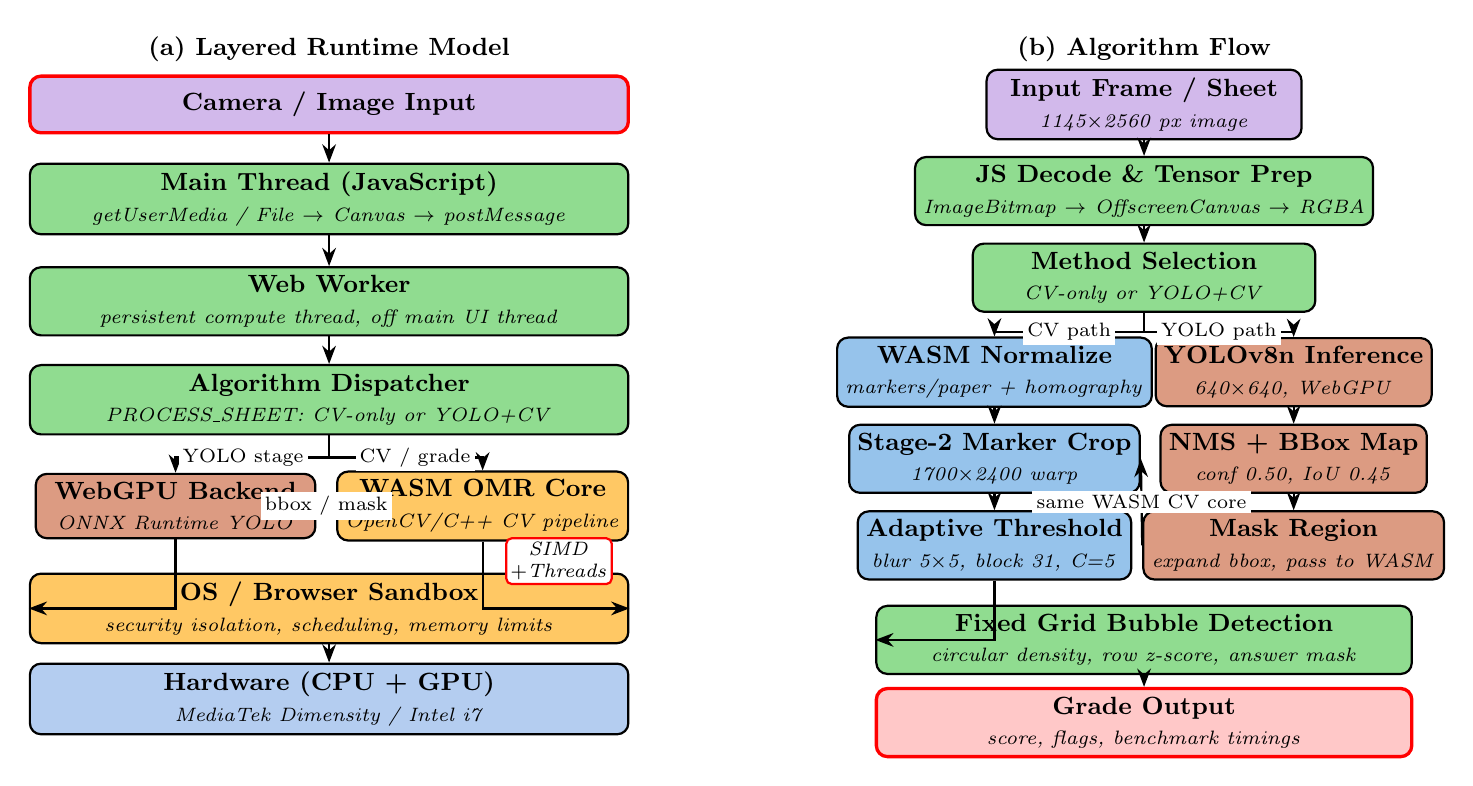
\begin{tikzpicture}[
  font=\small,
  >=Stealth,
  thick,
  every node/.style={align=center},
  base/.style    = {draw, rounded corners=4pt, text centered, inner sep=3pt},
  wide/.style    = {base, minimum width=7.6cm, minimum height=0.72cm},
  mid/.style     = {base, minimum width=3.55cm, minimum height=0.78cm},
  small/.style   = {base, minimum width=3.15cm, minimum height=0.70cm},
  camnd/.style   = {wide, fill=cpurple, draw=red, line width=1.2pt},
  wknd/.style    = {wide, fill=wgreen},
  dispnd/.style  = {wide, fill=wgreen, minimum height=0.88cm},
  osnd/.style    = {wide, fill=osbrown},
  hwnd/.style    = {wide, fill=hwblue},
  wgpund/.style  = {mid, fill=yorange},
  wasmnd/.style  = {mid, fill=osbrown},
  cfrnd/.style   = {base, fill=cpurple, minimum width=4.00cm, minimum height=0.72cm},
  jsnd/.style    = {base, fill=wgreen, minimum width=4.35cm, minimum height=0.72cm},
  cvbx/.style    = {small, fill=cblue},
  ylbx/.style    = {small, fill=yorange},
  mrgnd/.style   = {base, fill=wgreen, minimum width=6.8cm, minimum height=0.78cm},
  outnd/.style   = {base, fill=gpink, draw=red, line width=1.2pt,
                    minimum width=6.8cm, minimum height=0.68cm},
  simdlbl/.style = {draw=red, line width=0.8pt, fill=white,
                    rounded corners=2pt, inner sep=1.5pt, font=\scriptsize},
  lab/.style     = {fill=white, inner sep=1.5pt, font=\scriptsize}
]

%% ===== (a) Layered Runtime Model =====
\node[hwnd] (hw) at (0.00, 0.20)
  {\textbf{Hardware (CPU + GPU)} \\ \textit{\scriptsize MediaTek Dimensity / Intel i7}};
\node[osnd] (os) at (0.00, 1.35)
  {\textbf{OS / Browser Sandbox} \\ \textit{\scriptsize security isolation, scheduling, memory limits}};
\node[wasmnd] (wasm) at ( 1.95, 2.65)
  {\textbf{WASM OMR Core} \\ \textit{\scriptsize OpenCV/C++ CV pipeline}};
\node[wgpund] (wgpu) at (-1.95, 2.65)
  {\textbf{WebGPU Backend} \\ \textit{\scriptsize ONNX Runtime YOLO}};
\node[dispnd] (disp) at (0.00, 4.00)
  {\textbf{Algorithm Dispatcher} \\ \textit{\scriptsize PROCESS\_SHEET: CV-only or YOLO+CV}};
\node[wknd] (wk) at (0.00, 5.25)
  {\textbf{Web Worker} \\ \textit{\scriptsize persistent compute thread, off main UI thread}};
\node[wknd] (mt) at (0.00, 6.55)
  {\textbf{Main Thread (JavaScript)} \\
   \textit{\scriptsize getUserMedia / File $\to$ Canvas $\to$ postMessage}};
\node[camnd] (cam) at (0.00, 7.75)
  {\textbf{Camera / Image Input}};

\draw[->] (cam) -- (mt);
\draw[->] (mt) -- (wk);
\draw[->] (wk) -- (disp);
\draw[->] (disp.south) -- ++(0,-0.28) -| node[lab, pos=0.28] {YOLO stage} (wgpu.north);
\draw[->] (disp.south) -- ++(0,-0.28) -| node[lab, pos=0.28] {CV / grade} (wasm.north);
\draw[->, dashed] (wgpu.east) -- node[lab] {bbox / mask} (wasm.west);
\draw[->] (wgpu.south) -- ++(0,-0.36) |- (os.west);
\draw[->] (wasm.south) -- ++(0,-0.36) |- (os.east);
\draw[->] (os) -- (hw);
\node[simdlbl] at (2.92, 1.95) {\textit{SIMD} \\ +\textit{Threads}};

\node[font=\small\bfseries] at (0.00, 8.45) {(a) Layered Runtime Model};

%% ===== (b) Algorithm Flow =====
\node[cfrnd] (cfr) at (10.35, 7.75)
  {\textbf{Input Frame / Sheet} \\ \textit{\scriptsize 1145$\times$2560 px image}};
\node[jsnd] (decode) at (10.35, 6.65)
  {\textbf{JS Decode \& Tensor Prep} \\ \textit{\scriptsize ImageBitmap $\to$ OffscreenCanvas $\to$ RGBA}};
\node[jsnd] (select) at (10.35, 5.55)
  {\textbf{Method Selection} \\ \textit{\scriptsize CV-only or YOLO+CV}};

\node[cvbx] (cvnorm) at (8.45, 4.35)
  {\textbf{WASM Normalize} \\ \textit{\scriptsize markers/paper + homography}};
\node[cvbx] (stage2) at (8.45, 3.25)
  {\textbf{Stage-2 Marker Crop} \\ \textit{\scriptsize 1700$\times$2400 warp}};
\node[cvbx] (thr) at (8.45, 2.15)
  {\textbf{Adaptive Threshold} \\ \textit{\scriptsize blur 5$\times$5, block 31, C=5}};

\node[ylbx] (yolo) at (12.25, 4.35)
  {\textbf{YOLOv8n Inference} \\ \textit{\scriptsize 640$\times$640, WebGPU}};
\node[ylbx] (nms) at (12.25, 3.25)
  {\textbf{NMS + BBox Map} \\ \textit{\scriptsize conf 0.50, IoU 0.45}};
\node[ylbx] (mask) at (12.25, 2.15)
  {\textbf{Mask Region} \\ \textit{\scriptsize expand bbox, pass to WASM}};

\node[mrgnd] (grid) at (10.35, 0.95)
  {\textbf{Fixed Grid Bubble Detection} \\ \textit{\scriptsize circular density, row z-score, answer mask}};
\node[outnd] (grade) at (10.35, -0.10)
  {\textbf{Grade Output} \\ \textit{\scriptsize score, flags, benchmark timings}};

\draw[->] (cfr) -- (decode);
\draw[->] (decode) -- (select);
\draw[->] (select.south) -- ++(0,-0.24) -| node[lab, pos=0.25] {CV path} (cvnorm.north);
\draw[->] (select.south) -- ++(0,-0.24) -| node[lab, pos=0.25] {YOLO path} (yolo.north);
\draw[->] (cvnorm) -- (stage2);
\draw[->] (stage2) -- (thr);
\draw[->] (yolo) -- (nms);
\draw[->] (nms) -- (mask);
\draw[->] (mask.west) -- node[lab] {same WASM CV core} (stage2.east);
\draw[->] (thr.south) |- (grid.west);
\draw[->] (grid) -- (grade);

\node[font=\small\bfseries] at (10.35, 8.45) {(b) Algorithm Flow};

\end{tikzpicture}
  \caption{Updated Web-Based Edge OMR System Architecture. WebGPU accelerates only the YOLO localization stage; the deterministic OMR normalization, thresholding, bubble reading, and grading stages run through the WASM C++/OpenCV core.}
  \label{fig:arch}
\end{figure*}


% The system acquires the camera stream via \texttt{getUserMedia} and
% draws each frame on an off-screen \texttt{<canvas>}.
% Frames are dispatched to a Web Worker for multi-threaded processing so
% that the main UI thread remains responsive; results are returned to the
% main thread for real-time display.

% \subsection{Method 1: Traditional Computer Vision}

% The CV pipeline consists of three stages:
% \textbf{(i)}~pre-processing with grayscale conversion and Gaussian blur
% to reduce noise;
% \textbf{(ii)}~perspective correction using Canny edge detection to
% localize the paper frame, followed by a homography matrix $\mathbf{H}$
% for perspective warp; and
% \textbf{(iii)}~answer detection via adaptive thresholding, where the
% fill ratio is quantified by pixel density within each bubble region.

% \subsection{Method 2: Deep Learning with YOLO}

% We fine-tune YOLOv8n with four classes:
% \texttt{corner\_marker} (4 alignment marks at sheet corners),
% \texttt{info\_boundary} (student information and exam-code region),
% \texttt{questions\_1\_20}, and \texttt{questions\_21\_60}.
% Frames are resized to $640\times640$; after inference, non-maximum
% suppression (NMS) removes overlapping boxes, and detected bubble
% coordinates are mapped onto the paper grid to produce the final
% answer sheet.

% \subsection{Cross-Platform Deployment}

% Web Edge uses OpenCV.js (WASM) for CV and ONNX Runtime Web (WebGPU)
% for YOLO.
% OpenCV.js does not expose a GPU execution path; WASM is the only
% available backend for the CV pipeline in the browser, making the
% performance asymmetry between the GPU-accelerated YOLO stage and the
% CPU-bound CV stage a deployment constraint rather than a design choice.
% Native Android uses the OpenCV Android SDK (Kotlin + JNI) for CV and
% ONNX Runtime Android (CPU, 1~thread) for YOLO.
% Both OpenCV.js and the OpenCV Android SDK start from their respective
% default build configurations as unoptimised baselines; GPU-accelerated
% CV on Native (via OpenCL or Vulkan) and WASM SIMD+Threads on Web
% represent parallel optimisation paths applied asymmetrically in this
% study (Web SIMD+Threads is evaluated; Native GPU CV is not).
% We note that SIMD+Threads is applied to the Web CV pipeline but an
% equivalent GPU-accelerated CV path is not available for Native Android
% in this study; this asymmetry means that the Web optimisation frontier
% is more fully explored than the Native one, and the resulting
% Web--Native gap may be smaller than reported if Native CV were
% similarly accelerated (see Future Work, item~k).
% However, the directional conclusion that WASM execution overhead
% dominates is unlikely to be reversed by Native CV GPU optimisation:
% the WASM OMR stage ($1{,}124$\,ms) exceeds even the entire Native
% NNAPI E2E ($312$\,ms), so Native CV would need to reach near-zero
% latency before the optimisation asymmetry could alter the bottleneck
% attribution.
% Using the same \texttt{.onnx} file across Web and Native ensures a
% controlled cross-platform comparison, eliminating noise from
% framework-level model conversion; runtime-specific kernel optimisation
% by each backend is an inherent part of the deployment evaluation.
% The Web Edge Platform uses Python (opencv-python, PyTorch/CUDA).

\section{System Architecture and Methods}
\subsection{Architecture and Design Rationale}

The overall system architecture is illustrated in Fig.~\ref{fig:arch}. The system acquires camera frames via \texttt{getUserMedia}, renders them to an off-screen canvas, and dispatches processing to a Web Worker to preserve UI responsiveness during continuous inference. Fig.~\ref{fig:arch}(a) separates the runtime blocks from the algorithmic flow in Fig.~\ref{fig:arch}(b). The camera/image input block supplies either a live frame or an uploaded sheet image. The main JavaScript thread owns browser APIs, decodes the image through \texttt{ImageBitmap}/canvas, and sends the pixel buffer to the worker using \texttt{postMessage}. The worker contains the OMR pipeline state and an algorithm dispatcher that selects either the CV-only path or the YOLO+CV path for each sheet. When YOLO+CV is selected, the dispatcher invokes the algorithm flow in Fig.~\ref{fig:arch}(b), calls the WebGPU-backed ONNX Runtime session for localization, and then passes the resulting region to the same \wasm{} OMR core used by the CV-only path. The browser sandbox mediates both backends: JavaScript can request GPU execution only through WebGPU, while OpenCV-based CV functions execute as C\texttt{++} compiled to \wasm{} on CPU threads. The following design choices motivate the deployment architecture.

\textbf{CV+DL hybrid over CV-only.}
Pure CV pipelines are sensitive to perspective distortion, illumination variation, and partial occlusion~\cite{afifi2019}.
To improve robustness while remaining within mobile resource constraints, YOLOv8n is adopted for answer-region localization. The nano variant contains 3.2M parameters and requires 8.7~GFLOPs at $640\times640$, allowing deployment within the $\sim$50\,MB mobile VRAM budget while maintaining practical inference latency on WebGPU backends. Warm WebGPU inference remains within 142--299\,ms across evaluated devices; larger variants would increase inference cost proportionally with FLOPs, reducing interpretability of CV-stage latency analysis.

\textbf{\wasm{} for CV, WebGPU for DL.}
OpenCV.js currently exposes no browser-accessible GPU execution path; therefore, \wasm{} is the only available backend for the CV pipeline. In contrast, ONNX Runtime Web supports GPU acceleration through WebGPU for neural inference.
This heterogeneous execution model (shown in Fig.~\ref{fig:arch}(a)) is treated as a deployment constraint
rather than a design preference. Consequently, the performance asymmetry between CPU-bound \wasm{} execution and GPU-accelerated WebGPU inference forms a key focus of the latency analysis in Section~\ref{sec:latency}.

In the WebGPU path, JavaScript performs the host-side preparation before GPU execution: the worker letterbox-resizes the \texttt{ImageData} to $640\times640$ using an \texttt{OffscreenCanvas}, converts RGBA pixels into a normalized CHW \texttt{Float32Array}, and wraps the buffer as an ONNX Runtime tensor with shape $1\times3\times640\times640$. The session is created with the WebGPU execution provider, so convolutional YOLO kernels are scheduled through the browser's WebGPU layer rather than through direct native GPU APIs. After inference, JavaScript reads the output tensor, applies confidence filtering and NMS, maps the retained bounding box from letterbox coordinates back to the source frame, expands it, and forwards the masked/cropped region to the \wasm{} C\texttt{++}/OpenCV stage. Thus WebGPU accelerates only learned localization; thresholding, homography refinement, grid sampling, and grading remain in the deterministic \wasm{} path.

\textbf{Worker thread isolation.}
All frame processing is isolated from the UI thread through message-passing via \texttt{postMessage}.
Measured serialization overhead remains below 2\,ms and is small relative to end-to-end pipeline latency.

\subsection{Method 1: Traditional CV}

The traditional CV pipeline consists of three stages, illustrated in Fig.~\ref{fig:arch}(b). This path uses no learned detector; all decisions are made by deterministic image-processing and geometry rules. First, grayscale conversion and Gaussian blur are applied to suppress sensor noise and local intensity variation. Second, marker-corner detection is attempted using Otsu binarization, morphological opening, connected-component filtering, and quadrant assignment; if the marker path fails, a paper-boundary fallback estimates the outer sheet corners. The selected corners define a homography matrix $\mathbf{H}$ for perspective rectification, followed by a second marker-crop refinement into a canonical $1700\times2400$ sheet coordinate system. Third, a $5\times5$ Gaussian blur and adaptive mean thresholding (block size 31, $C=5$) are applied before fixed-grid analysis. Bubble centers are defined by the template grid, and each bubble is classified by foreground-pixel density inside a circular sampling window ($R=18$ px) with row-level normalization and suspicious-answer flags for ambiguous or multi-mark rows.

\subsection{Method 2: YOLOv8n + CV}

YOLOv8n is fine-tuned using four detection classes: \texttt{marker\_corners}, \texttt{id\_keycode}, \texttt{questions\_1\_20}, and \texttt{questions\_21\_60}, corresponding to the localization targets shown in Fig.~\ref{fig:arch}(b). The model is not trained from scratch: training starts from the pretrained \texttt{yolov8n.pt} weights and uses the four-class dataset configuration in \texttt{full\_label\_yolo/dataset.yaml}. The recorded training configuration uses $640\times640$ input images, 300 epochs with patience 80, batch size 8, AdamW optimization, initial learning rate 0.001, weight decay 0.0005, and geometric/photometric augmentation including rotation, translation, scale, shear, perspective, horizontal flip, mosaic, mixup, copy-paste, RandAugment, and random erasing. The exported \texttt{.onnx} model is then used unchanged by the Web and Android runtimes.

At inference time, the worker decodes the sheet image, letterbox-resizes it to $640\times640$, converts it to a normalized CHW tensor, and runs YOLOv8n. Candidate \texttt{marker\_corners} boxes are filtered at confidence 0.50 and NMS IoU 0.45. The retained box is mapped back to original image coordinates and expanded before masking/cropping the sheet region; the Web implementation uses 12\% expansion to avoid clipping edge markers, while the Android implementation uses 20\% expansion in the native benchmark. The cropped region is then passed to the same \wasm{}/native CV stages described above, so the learned component localizes the sheet region but does not directly classify bubbles.

\subsection{Cross-Platform Deployment}

\textbf{Web Edge:}
OpenCV.js (\wasm{}) is used for the CV pipeline, while ONNX Runtime Web (WebGPU backend) executes YOLO inference in Chrome v120+.

\textbf{Native Android:}
The OpenCV Android SDK (Kotlin + JNI) is used for CV processing, while ONNX Runtime Android executes YOLO inference under CPU (1T/4T) and NNAPI configurations.

\textbf{Deployment trade-offs:}
Desktop Web and Mobile Web share the same browser architecture and source code, but they differ in available memory bandwidth, thermal headroom, CPU scheduling, and sustained GPU frequency. Desktop Web therefore represents a zero-install deployment with relatively stable compute resources, whereas Mobile Web provides direct camera capture and installation-free field use but is constrained by battery, thermals, browser sandboxing, and limited background execution. Compared with a native mobile application, the Web version avoids app-store installation and keeps the same URL-deployed code across devices, but it cannot call OpenCV GPU backends directly and must execute C\texttt{++} CV through the \wasm{} memory model. Native Android has higher deployment friction and platform-specific packaging, but it can use JNI, native OpenCV, and NNAPI more directly, which explains the lower measured latency. Compared with server-side grading, both Web Edge and Native Android keep student sheets on the device and remove upload/network round trips; the Web Edge design specifically targets the case where privacy, connectivity, and installation friction are more limiting than raw compute throughput.

The same exported \texttt{.onnx} model is deployed across all platforms to reduce variance introduced by framework-specific model conversion. Runtime-specific kernel optimization performed by each backend is considered part of the deployment environment rather than an experimental confound. GPU-accelerated CV on Native Android (e.g., OpenCL or Vulkan backends) is not evaluated in this study, whereas \wasm{} SIMD+Threads optimization is evaluated for Web deployment. The implications of this optimization asymmetry are discussed in Section~\ref{sec:latency}.
% ============================================================
\section{Experimental Setup}

\subsection{System Environment}

\textit{Laptop}: Intel Core i7, 16\,GB RAM, Windows~11.
\textit{Mobile Device}: Xiaomi Redmi Note~13 Pro+
(MediaTek Dimensity~7200-Ultra, 8~cores, 8\,GB RAM,
Android~15, API~35).
\textit{Web Platform}: Chrome v120+ on both devices above. 

\subsection{Dataset}

All answer sheets follow the standard 60-question template used in
undergraduate courses at the University of Information Technology,
VNU-HCM (UIT-VNU), with five options (A/B/C/D/E) per question,
equivalent to 300 individual bubbles per sheet.
Images are captured at $1{,}145\times2{,}560$\,px with the rear
camera of a Xiaomi Redmi Note~13 Pro+.
The corpus is partitioned into two disjoint subsets serving distinct
roles in this study.

\textbf{(i) YOLO labeled set (detector training/validation).}
A subset of 56 sheets is manually annotated for the four detection
classes \texttt{marker\_corners}, \texttt{id\_keycode},
\texttt{questions\_1\_20}, and \texttt{questions\_21\_60}, and split
80/20 into 45 training and 11 validation images (see
\texttt{full\_label\_yolo/\{train,val\}.txt}).
The YOLOv8n detector is fine-tuned from the pretrained
\texttt{yolov8n.pt} weights for 176 epochs (early-stopped from a
300-epoch schedule with patience 80) using AdamW
($\mathrm{lr_0}{=}10^{-3}$, weight decay $5\times10^{-4}$, batch
size 8, image size $640$). Augmentation is applied on-the-fly by
the Ultralytics training loop and includes HSV jitter
($h{=}0.015$, $s{=}0.7$, $v{=}0.4$), rotation $\pm5^\circ$,
translation $\pm0.1$, scale $\pm0.3$, shear $\pm2^\circ$,
perspective $3\times10^{-4}$, horizontal flip $p{=}0.5$, mosaic
($p{=}1.0$, disabled for the last 10 epochs), MixUp $0.15$,
copy--paste $0.10$, RandAugment, and random erasing $0.4$.
The detector achieves $\mathrm{mAP}@0.5{=}0.995$ and
$\mathrm{mAP}@0.5{:}0.95{=}0.984$ on the held-out validation split.
The same exported \texttt{.onnx} weights are deployed unchanged on
all three runtime platforms.

\textbf{(ii) System evaluation set ($N{=}179$).}
A disjoint set of 179 sheets, organised into five sub-datasets
(\texttt{dataset\_1}\,$=48$, \texttt{dataset\_2}\,$=47$,
\texttt{dataset\_3}\,$=35$, \texttt{dataset\_4}\,$=45$,
\texttt{dataset\_5}\,$=4$), is used for all system-level evaluation.
The same 179-sheet set is replayed on Desktop Web, Mobile Web, and
Native Android, ensuring that latency, resource usage, and per-sheet
diagnostic measurements share identical inputs.
A subset of 100 sheets drawn from this set carries verified
ground-truth bitmasks (6{,}000 questions / 30{,}000 bubbles) and is
used for the question- and bubble-level accuracy comparison in
Section~\ref{sec:results-recognition}; the remaining sheets contribute
per-sheet diagnostic statistics (Section~\ref{sec:results-recognition}),
end-to-end latency (Section~\ref{sec:latency}), and resource
profiling (Section~\ref{sec:resources}).
Because the YOLO labeled set is not writer-disjoint from this
evaluation corpus, reported accuracy figures may be subject to writer
overlap; this limitation is discussed in
Section~\ref{sec:threats} (item vi).

\subsection{Evaluation Metrics}

\textbf{Accuracy} is computed at the question level: a question is
correct if and only if the system outputs the exact marked option
(A/B/C/D/E or ``blank'') matching the manual label.
With 100 sheets $\times$ 60 questions $= 6{,}000$ evaluation units,
accuracy is computed over 6,000 questions.
All 6,000 questions in the test set have exactly one option filled;
blank answers, which may arise in real examinations, are reserved for
future evaluation.
Precision, Recall, and F1 are reported at the bubble level over all
\textbf{30,000} individual bubbles (100 sheets $\times$ 300 bubbles)
to capture the two asymmetric error types: false positives (detecting a
mark on an empty bubble) and false negatives (missing a filled bubble).
We additionally report end-to-end inference time (ms/frame), peak CPU
usage (\%), and peak RAM usage (MB).
Throughout this paper, \emph{pipeline latency} refers to the processing
time from raw image file input to graded answer output, encompassing
JPEG decode, preprocessing, inference, post-processing, and a debug
JPEG write, but excluding camera acquisition and UI rendering.
JPEG decode is performed via different platform APIs (BitmapFactory on
Android; browser canvas pipeline on Web), and the debug write is
similarly platform-specific; however, both are included uniformly in
all reported E2E times on all configurations, so they contribute to
the absolute numbers but not to relative cross-platform ratios.
Based on stage measurements in Experiment~(d), combined I/O overhead
is $\approx$45\,ms on Native; an equivalent figure for Web is not
directly available, but the total processing gap exceeds 800\,ms
across all comparisons, making any plausible I/O difference
($<$50\,ms) immaterial to the reported ratios.
Throughout the paper, we distinguish between three levels of evidence:
\emph{directly measured} values (e.g., stage latencies from instrument\-ed
runs), \emph{derived estimates} (e.g., the counterfactual E2E projection),
and \emph{assumption-based extrapolations} (e.g., stage-ratio generalisation
to streaming); claims are interpreted with confidence appropriate to
their evidence level.

\textbf{CPU/RAM measurement.}
Because each platform exposes different telemetry APIs, we use the most
accurate tool for each environment:
Chrome Task Manager for Web---which reports CPU as a percentage of a
single logical core, so values above 100\% indicate use of more than
one core---\texttt{adb shell top} (out of 800\% for 8 cores) for
Native Android.
To mitigate heterogeneity we \textbf{(i)}~repeat each measurement over
all 100 test sheets and report peak values; \textbf{(ii)}~use identical
input images and identical order on all three platforms; and
\textbf{(iii)}~report results at the order-of-magnitude level
(e.g., ``$\sim10\times$'' vs.\ ``comparable'') so that qualitative
conclusions remain valid even under $\pm5$--$10\%$ measurement noise.

% ============================================================
\section{Results and Discussion}

\subsection{Recognition Accuracy}
\label{sec:results-recognition}

\subsubsection{Question-Level Accuracy}

Both pipelines---Traditional~CV and YOLO~+~CV (hybrid)---achieve
identical question-level accuracy of \textbf{96.4\%} over the 6{,}000
ground-truth-verified questions (Table~\ref{tab:accuracy},
$100$ sheets $\times$ $60$ questions).
This result confirms that introducing a YOLO-based region detector
into the OMR pipeline does not degrade recognition quality relative
to the purely traditional pipeline.

\subsubsection{Bubble-Level Detection Metrics}

At the bubble level over 30{,}000 individual bubbles
(Table~\ref{tab:confusion}), the two methods deliver comparable
overall performance but exhibit \emph{distinct error structures}.
Traditional~CV reaches Precision~$0.962$, Recall~$0.979$,
F1~$0.970$ (FN~$=126$, FP~$=234$), while YOLO~+~CV reaches
Precision~$\mathbf{0.983}$, Recall~$0.968$, F1~$\mathbf{0.975}$
(FN~$=192$, FP~$=102$).

\textbf{Error structure analysis.}
Traditional~CV tends to \emph{over-detect}: its adaptive thresholding
stage is sensitive to background noise, pencil smudges, and shadow
artefacts, producing a higher false-positive count.
YOLO~+~CV is more \emph{conservative}: the nano-scale model was
trained on clearly filled marks and remains cautious on faintly drawn
ones, reducing false positives at the cost of more false negatives.
In standardised examination grading, crediting an unanswered question
(a false positive) is generally considered more harmful to exam
integrity than missing a marked answer (a false negative) that can be
recovered during manual re-inspection.
Under this interpretation, the YOLO~+~CV error profile is the
preferable trade-off, though the final choice depends on each
institution's grading policy.

\subsubsection{YOLO Detection Performance}

The fine-tuned YOLOv8n detector achieves a 100\% \emph{region-level
detection rate}---every expected bounding box on the fixed template
is recovered---with mean confidence $\approx0.96$ consistently across
WebGPU (Chrome) and ONNX~Runtime~CPU (Android), confirming that the
detection stage does not introduce platform-dependent errors.
On the held-out validation split, the best epoch reaches
$\mathrm{mAP}@0.5{=}0.995$ and
$\mathrm{mAP}@0.5{:}0.95{=}\mathbf{0.984}$; the final epoch (176)
reports Precision~$0.993$, Recall~$1.000$.
This region-level detection metric is distinct from the bubble-level
classification metrics above: a bounding box can be correctly
localised yet still contain bubbles that are misclassified as filled
or empty during the downstream CV stage.
The high detection rate is partly attributable to the fixed,
repeated template structure; generalisation to alternative templates
is reserved for Future Work (item~g).

\begin{table}[t]
\caption{Question-Level Accuracy on the Test Set}
\label{tab:accuracy}
\centering
\begin{tabular}{lc}
\toprule
\textbf{Method} & \textbf{Accuracy (\%)} \\
\midrule
Traditional CV       & 96.4 \\
YOLO + CV (hybrid)   & 96.4 \\
\bottomrule
\end{tabular}
\end{table}
\begin{table}[t]
\caption{Bubble-Level Detection Metrics (30,000 Bubbles). Bold indicates the higher value per metric across the two methods.}
\label{tab:confusion}
\centering
\setlength{\tabcolsep}{3.5pt}
\begin{tabular}{lccccccc}
\toprule{}
\textbf{Method} & \textbf{TP} & \textbf{FP} & \textbf{FN} & \textbf{TN} & \textbf{P} & \textbf{R} & \textbf{F1} \\
\midrule{}
Traditional CV & 5,874 & 234 & 126 & 23,766 & 0.962          & \textbf{0.979} & 0.970          \\
YOLO + CV      & 5,808 & 102 & 192 & 23,898 & \textbf{0.983} & 0.968          & \textbf{0.975} \\
\bottomrule{}
\end{tabular}
\end{table}

\subsubsection{Diagnostic Analysis from Per-Sheet Data}

To complement the question- and bubble-level metrics, we extract
per-sheet diagnostic statistics from the full $N{=}179$ evaluation set
(Table~\ref{tab:diag}).
For each sheet we record the answered count, the number of suspicious
bubbles (intensity in the ambiguous grey-zone), the multi-mark count,
and an aggregate marker-alignment flag computed as
\mbox{$\texttt{marker\_fail}=\neg\texttt{keyValid}\land\neg\texttt{mssvValid}$}---a
sheet is flagged only when both the exam-code and the student-ID
checksums fail simultaneously, which is the strongest signal that
homography rectification has degraded both digit-bearing regions.

\begin{table}[t]
\caption{Per-Sheet Diagnostic Summary Across Five Sub-Datasets ($N{=}179$).}
\label{tab:diag}
\centering
\setlength{\tabcolsep}{3pt}
\begin{tabular}{lccccccc}
\toprule
\textbf{Sub-dataset} & \textbf{$N$} & \textbf{Avg Ans.}
  & \textbf{Full 60} & \textbf{Marker Fail}
  & \textbf{Avg Susp.} & \textbf{Avg Multi} & \textbf{$\Sigma$Multi} \\
\midrule
dataset\_1 & 48  & 58.98 & 13 & 0 (0.0\%) & 15.17 & 0.98 & 47 \\
dataset\_2 & 47  & 56.85 & 1  & 0 (0.0\%) & 22.81 & 0.70 & 33 \\
dataset\_3 & 35  & 56.89 & 6  & 0 (0.0\%) & 28.09 & 0.51 & 18 \\
dataset\_4 & 45  & 59.82 & 38 & 0 (0.0\%) & 23.31 & 0.04 & 2  \\
dataset\_5 & 4   & 60.00 & 4  & 0 (0.0\%) & 28.75 & 0.00 & 0  \\
\midrule
\textbf{Total} & 179 & 58.39 & 62 & 0 (0.0\%) & 22.05 & 0.56 & 100 \\
\bottomrule
\end{tabular}
\end{table}

Three observations emerge from this diagnostic data.

\textbf{(1) Marker alignment is robust on the evaluation corpus.}
No sheet in the 179-sheet evaluation set trips the
\texttt{marker\_fail} flag, i.e., every sheet yields at least one
valid Luhn-style checksum on either the exam-code or the student-ID
region.
This indicates that the homography produced from the four corner
markers is sufficiently accurate to correctly rectify both digit
regions on every input.
This finding does not, however, characterise behaviour on visibly
degraded sheets (e.g., extreme tilt, partial occlusion, severe
underexposure): such conditions are outside the current evaluation
corpus and are reserved for the writer-disjoint extension dataset
discussed in Section~\ref{sec:threats} (item vi).

\textbf{(2) Suspicious-bubble counts indicate grey-zone sensitivity.}
The average suspicious-bubble count is $22.05$ per sheet
(out of $60$ questions $\times$ $5$ options $=$ $300$ bubbles), but
the per-dataset spread is non-trivial: dataset\_1 averages $15.2$
while dataset\_3 and dataset\_5 reach $28.1$ and $28.8$
respectively.
A bubble is flagged ``suspicious'' when its fill ratio lies in the
ambiguous $[0.30,0.60]$ band, meaning the system must rely on
threshold-based tie-breaking rather than clear-cut classification.
The higher suspicious rate in dataset\_3 and dataset\_5 correlates
with lower full-60 counts (relatively low number of perfectly
answered sheets) and suggests these sub-datasets contain more
lightly-filled or photographically marginal sheets.

\textbf{(3) Multi-mark detections concentrate in the larger sub-datasets.}
A total of $100$ multi-mark events are observed across $179$
sheets ($0.56$ per sheet on average), but they are unevenly
distributed: dataset\_1 ($\Sigma{=}47$) and dataset\_2
($\Sigma{=}33$) together account for $80\%$ of all multi-mark
events, while dataset\_4 ($\Sigma{=}2$) and dataset\_5 ($\Sigma{=}0$)
are essentially clean.
Multi-mark events occur when the system detects more than one
filled option per question; they are often caused by faint stray
marks or by genuine multi-selection by the student rather than by
pipeline error.
The concentration in dataset\_1 and dataset\_2 suggests a
combination of larger sub-dataset size and a higher proportion of
informally-filled sheets in those collections.

\begin{figure}[t]
  \centering
  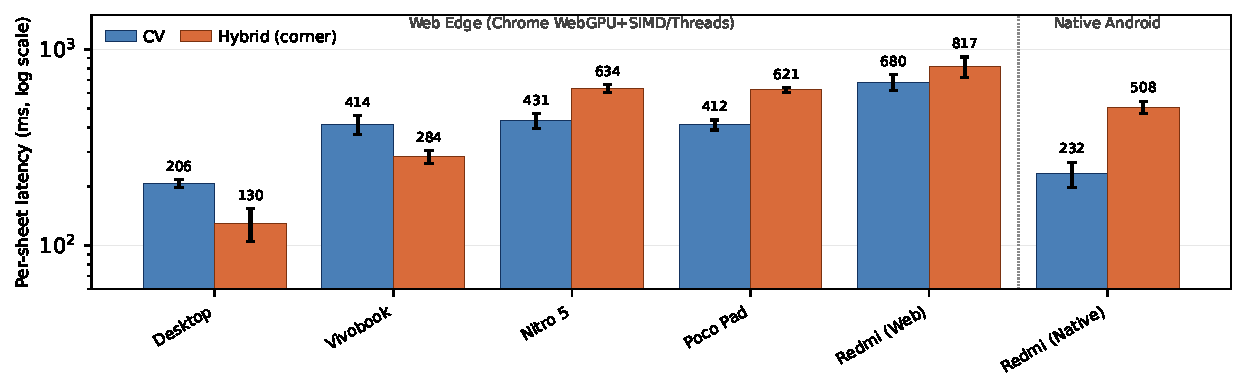
\includegraphics[width=\columnwidth]{figures/fig1_latency.pdf}
  \caption{End-to-End Latency by Platform and Configuration (ms, log scale).
  See Table~\ref{tab:latency} for footnotes on sample sizes and hardware.}
  \label{fig:latency}
\end{figure}

\subsection{Cross-Platform Latency}
\label{sec:latency}

Table~\ref{tab:latency} presents results in two measurement contexts.
The streaming context (top half) uses the original N=100 benchmark
and reflects full camera-stream application overhead.
The file-based context (bottom half) uses direct JPEG input to enable
a fair within-device comparison between Mobile Web SIMD and Native
Android across three provider configurations.
Three observations stand out.

\textbf{(1) WebGPU eliminates ML inference as the bottleneck.}
Warm WebGPU reduces YOLO inference from $1{,}170$\,ms (WASM warm) to
$142$\,ms---an $8.2\times$ speedup (Table~\ref{tab:stages}).
Yet end-to-end time does not drop proportionally because once YOLO is
offloaded to the GPU, the C++ OMR pipeline on the WASM thread becomes
the new bottleneck, accounting for $\sim$99\% of total time.

\textbf{(2) The real pipeline-level bottleneck is WASM OMR, not ML inference.}
In the file-based context---using identical JPEG inputs on both platforms---the
\emph{WASM OMR stage} ($1{,}124$\,ms) is $11\times$ slower than \emph{native
C++ OMR} ($\approx102$\,ms, measured directly from stage decomposition:
normalize~$80$\,ms, threshold~$17$\,ms, detect~$5$\,ms).
The WASM figure reflects the full cost of executing the same OpenCV algorithm
through the WebAssembly runtime, including JIT compilation artefacts,
WASM--JS boundary crossings, and linear-memory access patterns; the native
figure is pure C++ execution with no such overhead.
Because both implementations use identical OpenCV operations on identical
inputs, application-level implementation differences are limited to
platform-specific memory management and data layout; the
observed gap is therefore attributable primarily to the \emph{execution
environment}, not to algorithmic differences.
While we attribute the gap primarily to the execution environment,
residual contributions from implementation-level factors (memory
strategy, data transfer, scheduling) cannot be fully excluded.
Notably, closing this gap requires improvements to the WASM runtime
itself---such as WASM GC, memory64, or improved SIMD scheduling---rather
than changes to the OMR algorithm, placing it outside the direct control
of application developers.
Meanwhile, WebGPU YOLO inference ($299$\,ms) is only $2\times$ slower
than NNAPI ($168$\,ms).
Within the processing pipeline, this asymmetry is decisive: closing the OMR
gap would reduce Web YOLO E2E from $1{,}423$\,ms to $\approx401$\,ms,
leaving a $1.3\times$ pipeline-level difference driven solely by inference
backends.
A full file-based comparison shows Mobile Web SIMD YOLO
($1{,}423\pm163$\,ms) is $2.4\times$ slower than Native CPU-1T
($580\pm38$\,ms), $3.5\times$ slower than CPU-4T ($408\pm25$\,ms),
and $4.6\times$ slower than NNAPI ($312\pm23$\,ms), all under identical
input conditions.
All cross-platform pipeline-latency differences are statistically
significant (Welch's $t$-tests on independent samples drawn from the
same 100-sheet test set: $t>33$, $p<10^{-33}$ for all
Web-vs-Native pairs), confirming that the differences substantially exceed
measurement noise.
Because all configurations are evaluated on images drawn from the same
pool, cross-configuration measurements share input, which would support
a paired design if per-image Web SIMD timings were retained; they are
not, so Welch's test is used as a conservative alternative---adequate
given the large effect sizes.

\textbf{(3) On Native Android, adding YOLO costs no extra latency for this pipeline.}
In the streaming context, CV and YOLO reach nearly identical E2E
($2{,}362$\,ms vs.\ $2{,}231$\,ms): YOLO adds $429$\,ms for inference
but the bounding-box mask speeds up downstream bubble detection
($1{,}682$\,ms vs.\ $2{,}236$\,ms). The two trends cancel out for
this fixed-template, fixed-resolution dataset; this cancellation is
not guaranteed to hold for different question counts, layouts, or
model sizes where the inference cost may exceed the OMR speedup.

\begin{table}[t]
\caption{End-to-End Latency by Platform and Configuration (ms/frame)}
\label{tab:latency}
\centering
\resizebox{\columnwidth}{!}{%
\begin{tabular}{llcc}
\toprule
\textbf{Platform} & \textbf{Config} & \textbf{CV (ms)} & \textbf{YOLO (ms)} \\
\midrule
\multicolumn{4}{l}{\textit{Streaming context --- N=100, original benchmark}} \\
PC Web     & WebGPU                      & 6,389  & 16,472 \\
PC Web     & SIMD+Threads$^{*}$          &   540  &    643 \\
Mobile Web & WebGPU                      & 14,781 & 18,014 \\
Native     & ONNX CPU 1-thread           & 2,362  &  2,231 \\
\midrule
\multicolumn{4}{l}{\textit{File-based context --- N=43--56, JPEG I/O incl.}} \\
Mobile Web & SIMD+Threads$^{\dagger}$    & $1{,}090\pm152$ & $1{,}423\pm163$ \\
Native     & ONNX CPU 1-thread$^{\ddagger}$ & $207\pm33$   & $580\pm38$ \\
Native     & ONNX CPU 4-thread$^{\ddagger}$ & ---          & $408\pm25$ \\
Native     & ONNX + NNAPI$^{\ddagger}$      & ---          & $312\pm23$ \\
\bottomrule
\end{tabular}}
\vspace{2pt}
\parbox{\columnwidth}{\footnotesize
$^{*}$$N=54$, PC host (proof-of-concept; hardware differs from mobile).
$^{\dagger}$$N=50$ (CV) / $N=43$ (YOLO), Redmi Note~13 Pro+, Chrome Mobile, COOP/COEP.
$^{\ddagger}$$N=56$, Redmi Note~13 Pro+; E2E includes JPEG decode, full pipeline, and debug JPEG I/O ($\approx45$\,ms). Native CV uses OpenCV (provider-independent); CV time is identical across all three ONNX providers. JPEG decode is implemented differently across platforms (BitmapFactory on Android vs.\ browser canvas pipeline on Web), but the combined overhead is small relative to the processing gap and does not materially affect cross-platform comparisons.}
\end{table}

\begin{table}[!htbp]
\caption{YOLO Stage-Wise Latency Decomposition}
\label{tab:stages}
\centering
\resizebox{\columnwidth}{!}{%
\begin{tabular}{lcccc}
\toprule
\textbf{Backend} & \textbf{YOLO (ms)} & \textbf{\%E2E} & \textbf{OMR (ms)} & \textbf{E2E (ms)} \\
\midrule
WASM (cold)                  & 2,967     & $\sim$14\% & 17,948     & 21,004 \\
WASM (warm)                  & 1,170     & $\sim$12\% & 8,175      & 9,360  \\
WebGPU (warm)$^{\dagger\ddagger}$
                             & 142       & $\sim$1\%  & 16,839     & 16,472 \\
\midrule
WebGPU + SIMD+Threads$^{\S}$ & $81\pm12$ & $\sim$13\% & $438\pm11$ & $643\pm23$ \\
\midrule
\multicolumn{5}{l}{\textit{Mobile Web (Redmi Note~13 Pro+, COOP/COEP)}} \\
WebGPU + SIMD+Threads$^{\P}$ & $299\pm50$ & $\sim$21\% & ${\sim}1{,}124$ & $1{,}423\pm163$ \\
\bottomrule
\end{tabular}}
\vspace{2pt}

\parbox{\columnwidth}{\footnotesize
$^{\dagger}$E2E below stage sum due to async GPU dispatch.
$^{\ddagger}$Higher OMR under WebGPU reflects CPU throttling from GPU heat.
$^{\S}$PC host; OpenCV.js \texttt{-msimd128} + SharedArrayBuffer ($N=54$).
$^{\P}$Redmi Note~13 Pro+; Chrome Mobile; COOP/COEP ($N=43$).}
\end{table}

\textit{Thermal throttling.}
On PC Web (Chrome WebGPU), the first two frames run at near-ideal
speed (frame~2 reaches E2E~$=6{,}463$\,ms, almost matching the CV
baseline of 6,389\,ms, Table~\ref{tab:latency}).
From frame~3 onward, C++ OMR time climbs to $\sim$17,350\,ms and
stays elevated, consistent with thermal throttling.
Mobile Web throttles as early as frame~2 due to the limited thermal
headroom of smartphones.
Native Android shows no such decay: average E2E remains stable at
$1{,}966$\,ms (CV) and $2{,}758$\,ms (YOLO) across the entire test
set, consistent with the per-method values in Table~\ref{tab:latency}.
This sustained-workload performance decay is a web-specific limitation
for continuous image processing, and is the real bottleneck in many
scenarios---not the algorithm nor the ML back-end.

\textit{WebGPU cold-start.}
The WebGPU backend requires a one-time initialization (shader
compilation, model upload to VRAM) on the first frame: PC Web YOLO
frame~1 takes 1,771\,ms then drops to 74--142\,ms (warm); Mobile
frame~1 takes 926\,ms and drops to 226--711\,ms (warm).
This cost amortizes rapidly over longer grading sessions, making
WebGPU the right choice for bulk workflows.

\FloatBarrier
\subsection{Effect of SIMD and Multi-Threading on WASM Overhead}

To validate the hypothesis that WASM overhead is the addressable
bottleneck, we conduct a controlled SIMD+Threading experiment in
three complementary configurations.

\textbf{(a) PC reference (proof-of-concept).}
We rebuilt OpenCV.js with SIMD (\texttt{-msimd128}) and
SharedArrayBuffer multi-threading enabled, then re-ran the full
pipeline on the PC host using $N=54$ held-out answer sheets drawn
from an ongoing dataset extension (Chrome/Edge~147, Windows~10~x64).
The C++ OMR stage drops from $8{,}175$\,ms (WASM warm) to
$438\pm11$\,ms---an $\mathbf{18.7\times}$ reduction, far exceeding
the $2$--$3\times$ estimate based on SIMD alone.
The additional gain comes from multi-threading: perspective-warp and
adaptive-threshold stages are pixel-parallel and distribute efficiently
across cores via SharedArrayBuffer.
End-to-end latency falls to $540\pm20$\,ms (CV) and $643\pm23$\,ms
(YOLO).
This result is a PC-host upper bound on WASM optimisation headroom and
\emph{should not be compared directly with the mobile Native Android
baseline}, as the underlying hardware (desktop CPU vs.\ mobile SoC)
differs by an order of magnitude in compute throughput.

\textbf{(b) Mobile Web SIMD on the deployment device (within-device comparison).}
The same SIMD+Threads OpenCV.js build was served to the Redmi Note~13
Pro+ via Chrome Mobile, with the required
\texttt{Cross-Origin-Opener-Policy: same-origin} and
\texttt{Cross-Origin-Embedder-Policy: require-corp} headers to enable
SharedArrayBuffer.
On $N=50$ (CV) and $N=43$ (YOLO) held-out sheets (same template and
resolution as the main test set), the results are as follows.
CV end-to-end latency is $1{,}090\pm152$\,ms---a
$\mathbf{13.6\times}$ reduction from the unoptimised Mobile Web
baseline ($14{,}781$\,ms) and $2.2\times$ \emph{lower} than the
Native Android CV baseline ($2{,}362$\,ms) on the same device.
YOLO end-to-end latency is $1{,}423\pm163$\,ms---a
$\mathbf{12.7\times}$ reduction from the unoptimised baseline
($18{,}014$\,ms) and $1.6\times$ \emph{lower} than the Native
Android YOLO CPU baseline ($2{,}231$\,ms) on the same device.
The stage-wise breakdown for YOLO reveals that inference accounts for
$299\pm50$\,ms ($\sim$21\% of E2E) while the C++ OMR pipeline consumes
${\sim}1{,}124$\,ms ($\sim$79\%), confirming that the bottleneck
structure identified on PC Web (Table~\ref{tab:stages}) generalises
to Mobile Web under SIMD optimisation.
Thermal throttling is more pronounced than on PC: the first-five-to-last-five
frame delta is $+207$\,ms for CV and $+298$\,ms for YOLO, consistent
with the narrower thermal headroom of the mobile SoC under sustained
WebGPU+WASM load.

\textbf{(c) Native Android with NNAPI (hardware-accelerated baseline).}
For the YOLO path, we additionally evaluate ONNX Runtime Android with
the NNAPI execution provider (FP16 disabled), which delegates inference
to the Dimensity~7200-Ultra hardware accelerator.
On $N=56$ sheets with a 5-sheet warm-up and ORT timing corrected via
\texttt{SystemClock.elapsedRealtime()} with forced tensor materialisation,
YOLO ORT time drops from $385\pm17$\,ms (CPU 1-thread) to
$168\pm15$\,ms (NNAPI)---a $\mathbf{2.3\times}$ speedup.
The NNAPI pass shows no thermal runaway (last--first E2E delta
$-47$\,ms, \emph{improving} as the GPU scheduler warms up),
in contrast to the CPU 1-thread pass ($+33$\,ms delta).
Full-pipeline E2E on file-based input ($N=56$, JPEG I/O included)
reaches $580\pm38$\,ms (CPU 1-thread), $408\pm25$\,ms (CPU 4-thread),
and $312\pm23$\,ms (NNAPI); the native OMR stage accounts for
$195$\,ms, $191$\,ms, and $144$\,ms respectively (measured as
E2E~$-$~ORT, including bitmapToMat and debug JPEG write,
$\approx45$\,ms/sheet).

\textbf{(d) Native Android CV file-based benchmark.}
To complete the within-device comparison and directly measure native
C++ OMR speed, we run the pure OpenCV pipeline on $N=56$ sheets (same
dataset, no YOLO inference) with the same JPEG I/O framing.
End-to-end latency is $207\pm33$\,ms, with a stage breakdown of:
JPEG decode~$26$\,ms, bitmap conversion~$10$\,ms,
perspective warp (NormalizePaper)~$80$\,ms, Otsu threshold~$17$\,ms,
bubble detection~$5$\,ms, and debug JPEG write~$63$\,ms.
The \emph{pure C++ OMR computation} (warp + threshold + detect) totals
$\approx102$\,ms---matching the estimate used in the counterfactual
analysis---while I/O overhead accounts for the remaining $\approx100$\,ms.
Thermal drift is nominal (last--first E2E delta $+44$\,ms).

\textbf{(e) Native Android streaming stage decomposition.}
A supplementary streaming simulation ($N=54$) loads each sheet as a
full-resolution Bitmap---mimicking the Android camera output format---and
measures: frame load~$60\pm15$\,ms, CV processing~$181\pm27$\,ms,
debug write~$12\pm7$\,ms; total $255\pm39$\,ms.
Comparing with the streaming-context Native baseline ($2{,}362$\,ms,
Table~\ref{tab:latency}), camera acquisition and Android camera2 API
overhead account for the majority of the streaming gap ($\approx2{,}100$\,ms),
not the processing pipeline itself.

\textbf{Combined interpretation.}
Three findings emerge from the optimised configurations.
\emph{First}, in the file-based context, Mobile Web SIMD YOLO
($1{,}423\pm163$\,ms) is $2.4\times$, $3.5\times$, and $4.6\times$
slower than Native CPU-1T ($580\pm38$\,ms), CPU-4T ($408\pm25$\,ms),
and NNAPI ($312\pm23$\,ms) respectively---a substantial improvement
over the unoptimised baseline ($18{,}014$\,ms, $12.7\times$ reduction)
but not a reversal of the Web--Native order.
The performance gap is driven by the OMR pipeline:
WASM OMR ($1{,}124$\,ms) is $11\times$ slower than native C++ OMR
($\approx102$\,ms, measured directly via stage decomposition in
experiment~(d)), whereas WebGPU YOLO ($299$\,ms) is only $2\times$
slower than NNAPI ($168$\,ms).
For the CV path, Mobile Web SIMD ($1{,}090\pm152$\,ms) is $5.3\times$
slower than Native CV ($207\pm33$\,ms), independently corroborating
that WASM overhead dominates even in the absence of deep learning
inference---confirming that the bottleneck is architectural, not
model-dependent.
We note that this stage-level attribution is derived from file-based
measurements; we assume that the relative stage contributions
generalise to the streaming pipeline, although this cannot be
directly verified for Web due to the lack of streaming-context
stage instrumentation.
\emph{Second}, if WASM OMR could reach native C++ speed ($\approx102$\,ms),
the residual Web YOLO E2E would fall to $\approx401$\,ms---only
$1.3\times$ above NNAPI ($312$\,ms). This illustrates that WASM OMR
overhead is the \emph{primary driver of the pipeline-level latency
difference} (measured under identical input conditions); closing it
would reduce the pipeline gap to a level dominated by inference-backend
differences.
This is a first-order estimate treating additive stage contributions
as the baseline scenario; it yields a \emph{lower bound on achievable
improvement}, because any thermal relief from reducing CPU-bound OMR
load would further decrease GPU inference latency beyond the
$1.3\times$ figure.
The estimate does not assume strict component independence; rather,
it provides the most conservative scenario (no coupling benefit),
with the understanding that real-world coupling can only improve
the outcome.
\emph{Third}, the bottleneck structure is robust: even with SIMD+Threads,
the OMR pipeline accounts for $\sim$79\% of YOLO E2E on Mobile Web
($1{,}124$ of $1{,}423$\,ms), while on Native it accounts for only
$\sim$46\% ($144$ of $312$\,ms under NNAPI, including $\approx45$\,ms
I/O overhead; pure C++ OMR $\approx102$\,ms, or $\sim$33\% of
NNAPI E2E)---making the OMR stage the single largest determinant of
the pipeline-level latency difference across platforms.
Within Native Android (same $N=56$ sheets), paired $t$-tests confirm
that CPU-4T is significantly faster than CPU-1T ($t=30.3$,
$p<10^{-35}$), and NNAPI significantly faster than CPU-4T
($t=22.6$, $p<10^{-28}$).
The file-based context is an \emph{isolation measurement} of the
processing pipeline; it does not include camera acquisition,
\texttt{canvas} rendering, or UI-thread overhead present in streaming
deployment, and should not be interpreted as a system-level
end-to-end evaluation.

\subsection{System Resource Usage}
\label{sec:resources}

System resource consumption was measured on all three platforms
during the $N{=}179$ benchmark run, covering both the Traditional~CV
and YOLO~+~CV pipelines.
Table~\ref{tab:resources} summarises peak values; per-sheet
time-series are visualised in
Figs.~\ref{fig:cpu_cv}--\ref{fig:cross_platform}.

\begin{table}[!h]
\caption{System Resource Usage Summary ($N{=}179$)}
\label{tab:resources}
\centering
\resizebox{\columnwidth}{!}{%
\begin{tabular}{lcccc}
\toprule
\textbf{Platform} & \textbf{CPU-CV} & \textbf{RAM-CV (MB)}
  & \textbf{CPU-YOLO} & \textbf{RAM-YOLO (MB)} \\
\midrule
PC Web          & $\sim$1.46$^{a}$ & $\sim$505 & $\sim$0.99$^{a}$ & $\sim$249 \\
Mobile Web      & $\sim$1.62$^{a}$ & $\sim$156 & $\sim$1.59$^{a}$ & $\sim$156 \\
Native Android  & $\sim$539$^{b}$  & $\sim$485 & $\sim$497$^{b}$  & $\sim$624 \\
\bottomrule
\end{tabular}}
\vspace{2pt}
\parbox{\columnwidth}{\footnotesize
$^{a}$Web CPU reported as the event-loop \texttt{cpu\_load\_proxy}
(fraction of one logical core; $1.0=$ saturated single core).
$^{b}$Android CPU reported by \texttt{adb shell top}
(out of $800\%$ for $8$ cores).
CPU measurement instruments differ across platforms; values are
reported for within-platform comparison only.}
\end{table}

\subsubsection{CPU Usage}

\begin{figure}[t]
  \centering
  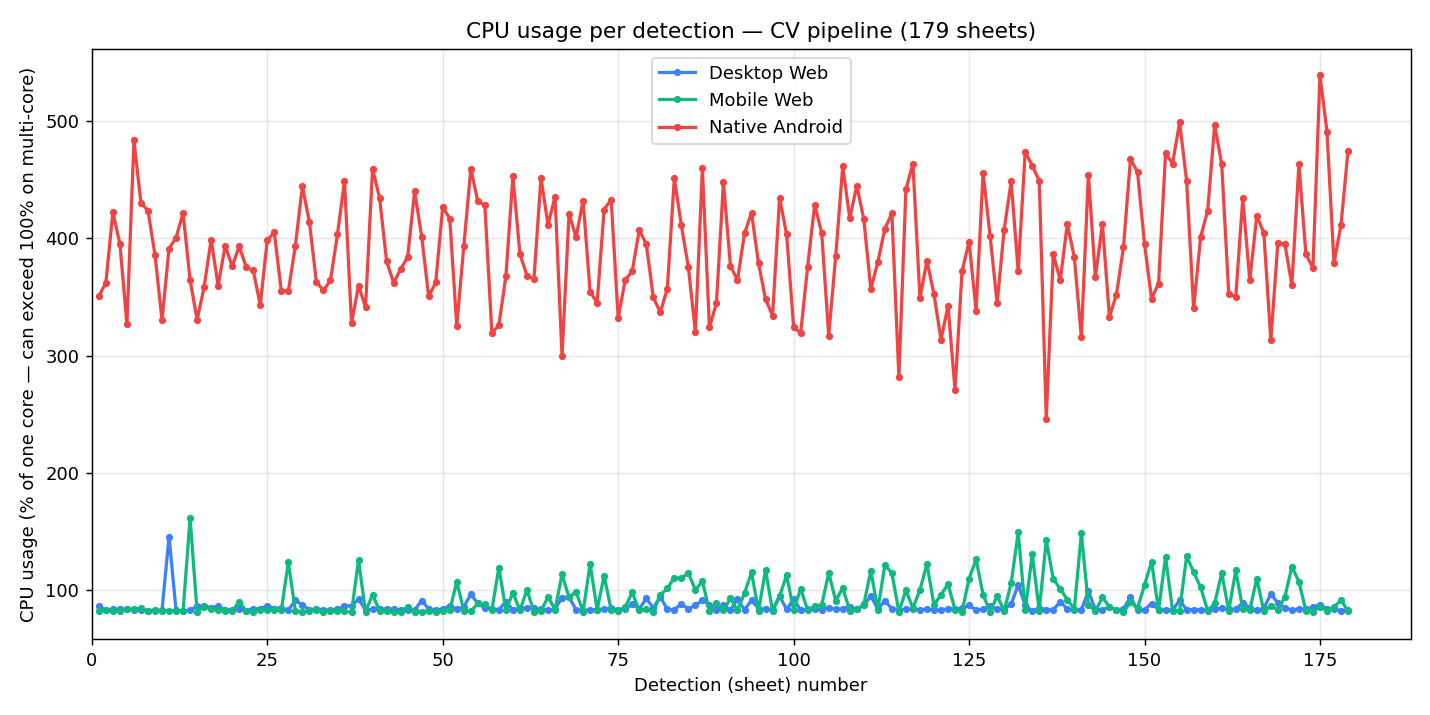
\includegraphics[width=\columnwidth]{figures/chart_cpu_cv.png}
  \caption{CPU usage per detection---Traditional CV pipeline
  ($N{=}179$). Native Android (red) sustains $300$--$500\%$
  utilisation across multiple cores, while both Web platforms
  (blue, green) remain at or below $\sim\!100\%$ of a single core,
  constrained by the single-threaded WASM execution model.}
  \label{fig:cpu_cv}
\end{figure}

\begin{figure}[t]
  \centering
  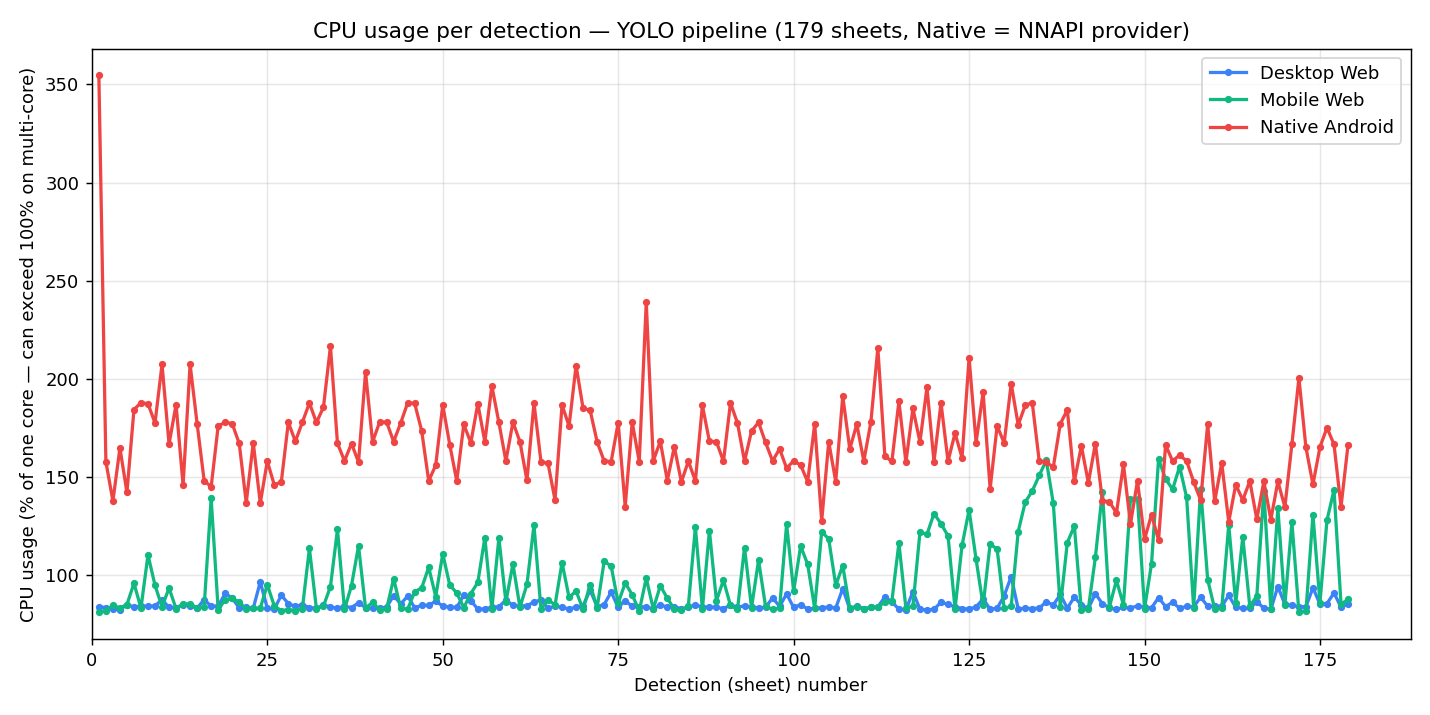
\includegraphics[width=\columnwidth]{figures/chart_cpu_yolo.png}
  \caption{CPU usage per detection---YOLO~+~CV pipeline
  ($N{=}179$). Native Android CPU drops to $150$--$200\%$
  (from $300$--$500\%$ for CV-only) because WebGPU / NNAPI
  offloads inference to the GPU/NPU, reducing CPU-side work.}
  \label{fig:cpu_yolo}
\end{figure}

\textbf{Traditional CV pipeline---three platforms.}
On PC~Web, the CV pipeline reaches a peak CPU load proxy of
$\sim\!1.46$ (i.e., $\sim\!146\%$ of one core), averaging
$\sim\!0.65$ during sustained processing.
Mobile~Web shows a similar pattern, peaking at $\sim\!1.62$.
As shown in Fig.~\ref{fig:cpu_cv}, both Web traces remain flat near
the $100\%$ line across all 179 sheets, confirming that the WASM
runtime executes on a single main thread with minimal parallelism.
On Native~Android, the CV pipeline peaks at $\sim\!539\%$ (out of
$800\%$ on the 8-core Dimensity~7200-Ultra), averaging $\sim\!349\%$.
The high-variance oscillation in the Native trace reflects OpenCV's
native multi-threading distributing pixel-parallel operations
(perspective warp, adaptive thresholding) across cores in bursts.
\emph{Take-away.}
The WASM execution model caps Web at $\le2$ logical cores
regardless of available hardware parallelism, whereas Native
Android utilises the full SoC core complement.

\textbf{YOLO~+~CV pipeline---three platforms.}
On PC~Web, the YOLO pipeline peaks at $\sim\!0.99$---lower than CV
because WebGPU offloads inference to the GPU, reducing CPU
contention.
Mobile~Web shows a similar peak of $\sim\!1.59$.
On Native~Android, the YOLO pipeline peaks at $\sim\!497\%$ with an
average of $\sim\!226\%$, notably lower than the CV-only average
($\sim\!349\%$).
This reduction is clearly visible when comparing
Fig.~\ref{fig:cpu_yolo} with Fig.~\ref{fig:cpu_cv}: the Native trace
drops from the $300$--$500\%$ band to the $150$--$200\%$ band,
because the YOLO bounding-box mask reduces the pixel area that the
downstream CV stage must process.
\emph{Take-away.}
GPU/NPU inference offload (WebGPU on Web, NNAPI on Native) shifts
CPU work to the accelerator and, on Native, the bounding-box mask
further reduces downstream CPU load.

\textbf{Overall CPU conclusion.}
Lower Web CPU usage is \emph{not} an efficiency advantage but a
\emph{constraint} of the single-threaded WASM execution model;
Native Android exchanges substantially higher CPU utilisation
($2$--$4\times$) for proportionally higher throughput, and the
YOLO~+~CV pipeline is more CPU-efficient than CV-only on Native
because the detector mask reduces downstream pixel work.

\subsubsection{RAM Usage}

\begin{figure}[t]
  \centering
  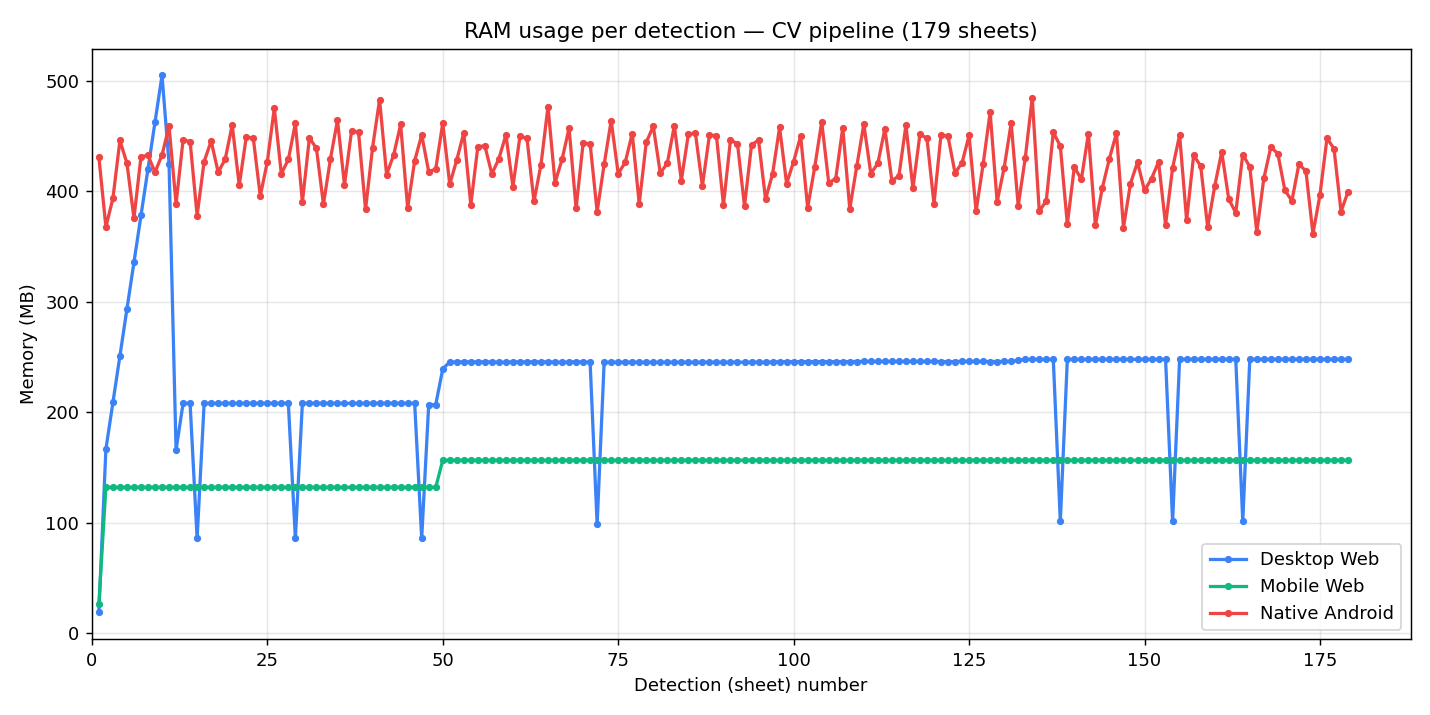
\includegraphics[width=\columnwidth]{figures/chart_ram_cv.png}
  \caption{RAM usage per detection---Traditional CV pipeline
  ($N{=}179$). PC Web (blue) shows a staircase pattern as the WASM
  linear memory grows in fixed increments, peaking at $\sim\!505$\,MB
  around sheet~10 before stabilising. Mobile Web (green) plateaus at
  $\sim\!156$\,MB constrained by a lower \texttt{js\_heap\_limit}.
  Native Android (red) oscillates between $370$--$485$\,MB, driven by
  cyclic native-heap allocation of per-image OpenCV buffers.}
  \label{fig:ram_cv}
\end{figure}

\begin{figure}[t]
  \centering
  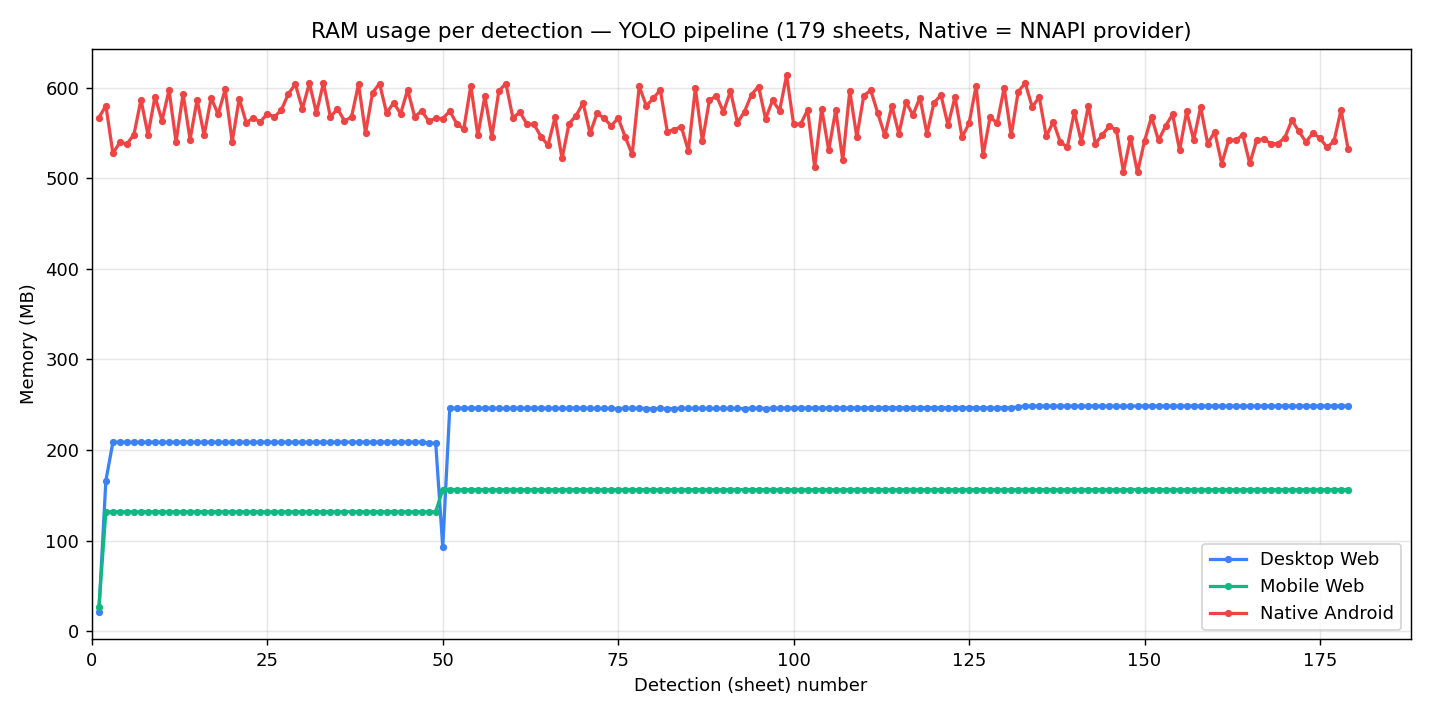
\includegraphics[width=\columnwidth]{figures/chart_ram_yolo.png}
  \caption{RAM usage per detection---YOLO~+~CV pipeline
  ($N{=}179$). Native Android shifts upward to the $520$--$624$\,MB
  band due to the ONNX~Runtime and model weights
  ($+\sim\!139$\,MB vs.\ CV). PC Web stabilises at
  $\sim\!210$--$249$\,MB (smaller dedicated YOLO WASM module).
  Mobile Web remains at $\sim\!156$\,MB.}
  \label{fig:ram_yolo}
\end{figure}

\textbf{Traditional CV pipeline---three platforms.}
PC~Web records the highest peak memory at $\sim\!505$\,MB
(JS~heap~$+$~WASM~heap), driven by the large WASM linear-memory
allocation that grows in fixed increments during the first
$\sim\!10$ sheets before stabilising
(Fig.~\ref{fig:ram_cv}).
Mobile~Web peaks at $\sim\!156$\,MB, constrained by the lower
\texttt{js\_heap\_limit} ($\sim\!1{,}078$\,MB on the test device
vs.\ $\sim\!4{,}096$\,MB on desktop); its trace is essentially flat
across the run, indicating that memory allocation saturates early
and does not grow with workload.
Native~Android peaks at $\sim\!485$\,MB RSS (JVM heap $\sim\!93$\,MB
plus native heap up to $\sim\!223$\,MB); the oscillating pattern
reflects cyclic allocation and deallocation of per-image OpenCV
buffers within each detection cycle.
\emph{Take-away.}
WASM linear memory dominates the Web RAM footprint and is
input-independent, whereas Native Android RAM tracks the per-image
working set cyclically.

\textbf{YOLO~+~CV pipeline---three platforms.}
On PC~Web, adding the YOLO model lowers the peak to $\sim\!249$\,MB
because the YOLO and CV pipelines run in separate WASM modules and
only one is active at a time during measurement.
Mobile~Web peaks at $\sim\!156$\,MB, identical to CV.
On Native~Android, the YOLO pipeline adds $\sim\!139$\,MB over the
CV baseline, raising peak RSS to $\sim\!624$\,MB
(native heap up to $\sim\!342$\,MB, JVM heap up to $\sim\!130$\,MB);
the additional memory is attributable to the ONNX~Runtime and the
model weights loaded into the native heap.
\emph{Take-away.}
The ONNX~Runtime + model contribute a consistent $\sim\!139$\,MB
overhead on Native, while Web platforms see no such increase
because each pipeline uses its own WASM module.

\textbf{Overall RAM conclusion.}
Web RAM is dominated by the WASM linear-memory architecture rather
than by the workload or by the addition of YOLO; Native RAM scales
with the working set and the ONNX~Runtime footprint.
All measured peaks remain well within the capacity of mid-range
devices ($\ge 8$\,GB RAM), but the staircase Web allocation pattern
may pose problems on low-end devices with $<\!4$\,GB RAM where the
OS may terminate the browser tab under memory
pressure~\cite{androidmarket2024}.

\subsubsection{Combined Resource Efficiency}

\begin{figure}[t]
  \centering
  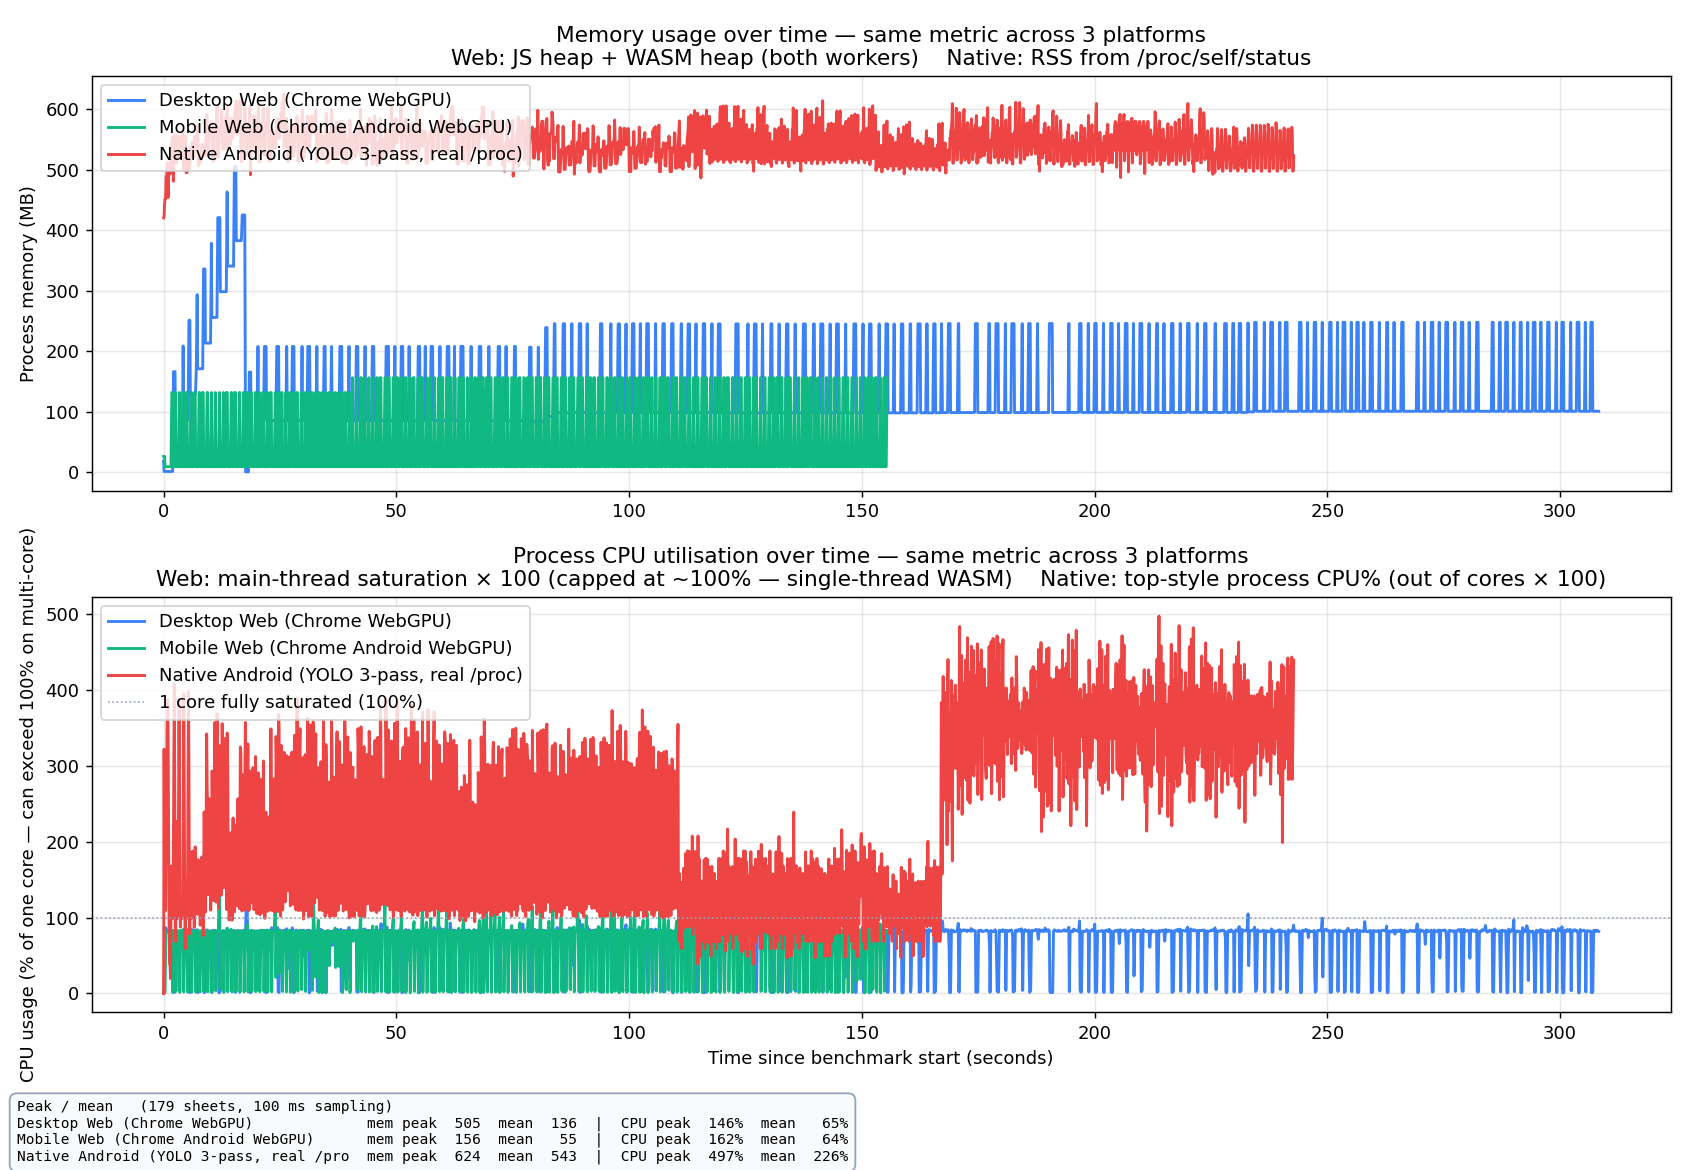
\includegraphics[width=\columnwidth]{figures/chart_cross_platform.png}
  \caption{Combined memory (top) and CPU (bottom) over time across
  all three platforms. The plot confirms the two dominant patterns:
  (i) Web memory stabilises early and remains flat, while Native
  oscillates with per-image buffer cycles; (ii) Native CPU saturates
  multiple cores while Web remains near single-core capacity.}
  \label{fig:cross_platform}
\end{figure}

Fig.~\ref{fig:cross_platform} provides an integrated view of CPU
and memory utilisation over time.
\textbf{Native~Android} achieves the best resource-to-performance
ratio of the three platforms: it utilises multiple cores effectively
(up to $\sim\!539\%$ CPU), maintains a moderate memory footprint
($\sim\!485$--$624$\,MB), and delivers the lowest end-to-end latency
($207$--$580$\,ms depending on configuration, see
Section~\ref{sec:latency}).
\textbf{Web platforms}, constrained by the single-threaded WASM
execution model and linear-memory allocation, consume fewer CPU
cycles but achieve proportionally lower throughput, with memory
usage dominated by architectural overhead rather than
application-level data.
The \textbf{YOLO~+~CV pipeline} is more resource-efficient than the
pure CV pipeline on Native (CPU avg $226\%$ vs.\ $349\%$, $+139$\,MB
RAM), because the detector bounding-box mask reduces the pixel area
processed by the downstream CV stage; on Web, this efficiency
benefit is masked by the dominant WASM execution overhead.
These resource characteristics should be weighed alongside the
latency findings when selecting a deployment platform: Native
Android offers both higher throughput and a more predictable
resource profile, while Web deployment trades performance for
broader reach---subject to the RAM-availability constraint noted
above.



\textbf{Threats to validity.}
\label{sec:threats}
\begin{enumerate}[label=(\roman*), leftmargin=*, itemsep=2pt, topsep=4pt]
  \item CPU/RAM measurement tools differ across platforms; we mitigate
    by reporting only order-of-magnitude trends.
  \item Results were obtained on a Redmi Note~13 Pro+ with Chrome;
    iOS/Safari evaluation is deferred to future work (Section~VI,
    item~a). Secondary tests on a Samsung Galaxy~A15 (Chrome, WebGPU)
    confirm the Web--Native ratio ($7.0\times$ and $8.3\times$ for CV
    and YOLO); Firefox without WebGPU increases YOLO E2E to 24,186\,ms
    vs.\ 16,472\,ms with Chrome WebGPU, underscoring the Chromium
    dependency.
  \item The long-run slow-down on Web may combine thermal throttling,
    background-tab throttling, and garbage collection; CPU temperature
    was not measured directly and results are therefore reported as
    ``consistent with thermal throttling.''
  \item The baseline OpenCV.js build uses no SIMD or multi-threading.
    Section~V-C reports a SIMD+Threads experiment reducing the OMR
    stage by $18.7\times$; the bottleneck conclusion holds across both
    build configurations, with OMR remaining the dominant cost.
  \item The streaming-context Native Android baseline (Table~\ref{tab:latency},
    top half) uses ONNX Runtime CPU 1-thread. A file-based benchmark
    ($N=56$, same device, ORT timer corrected via forced tensor
    materialisation) measures full-pipeline E2E for CPU 1-thread
    ($580\pm38$\,ms), CPU 4-thread ($408\pm25$\,ms), and NNAPI
    ($312\pm23$\,ms), as well as pure CV ($207\pm33$\,ms), providing
    fair within-context comparisons against Mobile Web SIMD
    ($1{,}090\pm152$\,ms CV, $1{,}423\pm163$\,ms YOLO).
    The two measurement contexts (streaming vs.\ file-based) are not
    directly comparable due to differing overheads (camera acquisition
    accounts for $\approx2{,}100$\,ms of the streaming-context total,
    as shown by the streaming stage decomposition in Section~V-C\,(e));
    results from each context are interpreted within that context only.
  \item All sheets in the corpus are captured on a single device
    (Redmi Note~13 Pro+), and the YOLO labeled set is not strictly
    disjoint from the 179-sheet system evaluation set in terms of
    writers. The detector may therefore have been exposed to the
    handwriting style, pen pressure, and mark-intensity distribution
    of evaluation writers during training, potentially inflating the
    reported 96.4\% accuracy.
    The magnitude of this inflation is unknown without a writer-disjoint
    experiment; generalisation to unseen writers, diverse devices, and
    adverse lighting is not yet validated.
    A writer-disjoint dataset is in preparation.
  \item The YOLO detector is trained on only 56 manually annotated
    sheets ($45$ train, $11$ val). While augmentation
    (Section~III, Dataset) expands the effective sample diversity,
    the small label budget combined with the fixed-template structure
    biases the model toward learning anchor positions rather than
    template-agnostic region features. Generalisation to alternative
    answer-sheet templates is not validated and is reserved for
    Future Work.
  \item Energy consumption and battery draw were not measured.
    Running WebGPU alongside multi-threaded WASM is expected to consume
    significantly more power than an equivalent native pipeline;
    energy efficiency is a critical metric for edge deployment and
    its omission limits the practical conclusions that can be drawn
    from the latency results alone.
  \item All Web and Native measurements are conducted on a single
    device (Redmi Note~13 Pro+, MediaTek Dimensity~7200-Ultra).
    WebGPU performance, WASM throughput, and NNAPI behaviour depend
    heavily on GPU driver, browser version, and SoC vendor; results
    on Qualcomm, Samsung Exynos, or Apple A-series hardware may differ
    substantially. The findings should be interpreted as
    device-specific rather than platform-universal until replicated
    across additional hardware.
  \item All benchmarks use a fixed input resolution ($1{,}145\times2{,}560$\,px)
    and a single answer-sheet template (60-question, 4-option grid).
    The observed bottleneck structure---WASM OMR dominating at $\sim$79\%
    of E2E---may shift under different resolutions, question counts, or
    answer layouts, as these affect the relative cost of the perspective-warp
    and bubble-detection stages. Conclusions regarding bottleneck dominance
    are therefore confined to the evaluated configuration.
\end{enumerate}

% ============================================================
\section{Conclusion}

This paper presents a \emph{pipeline-level} benchmark of a
browser-based OMR system---measuring processing latency from decoded
image to graded answer, on a single mid-range Android device (Redmi
Note~13 Pro+)---across three execution stacks and six build
configurations.
\begin{enumerate}[leftmargin=*, itemsep=2pt, topsep=4pt]
  \item Both CV and YOLO reach \textbf{96.4\%} per-question accuracy.
    Error structures differ: CV over-detects (FP~$=234$, FN~$=126$)
    while YOLO is more conservative (FP~$=102$, FN~$=192$).
    In grading contexts where a false positive (crediting an unanswered
    question) is considered more harmful than a false negative,
    YOLO's error profile is preferable; this trade-off is
    institution-dependent.
  \item WebGPU reduces warm YOLO inference by $8.2\times$
    ($1{,}170\to142$\,ms). In the file-based benchmark, Native full-pipeline
    E2E is $580\pm38$\,ms (CPU 1-thread), $408\pm25$\,ms (CPU 4-thread),
    and $312\pm23$\,ms (NNAPI), and Native CV is $207\pm33$\,ms---all
    substantially faster than Mobile Web
    SIMD YOLO ($1{,}423\pm163$\,ms). The $2.4$--$4.6\times$ pipeline-level
    latency difference (under identical input conditions) is driven by WASM
    OMR ($1{,}124$\,ms) being $11\times$ slower than native C++ OMR
    ($\approx102$\,ms, directly measured), not by the inference backends.
    Notably, the CV-only comparison independently confirms this: Mobile Web
    SIMD CV ($1{,}090$\,ms) is $5.3\times$ slower than Native CV ($207$\,ms),
    demonstrating WASM overhead dominates even without deep learning inference.
  \item Without SIMD, the $2.7$--$8.1\times$ end-to-end gap between
    Web Edge and Native Android stems from the C++ OMR pipeline running
    through WebAssembly, not from ML inference---the YOLO stage accounts
    for only $\sim$1\% of total time once WebGPU is used.
  \item Enabling SIMD and multi-threading in OpenCV.js reduces the C++
    OMR stage by $18.7\times$ on a PC host and brings Chrome-based Mobile
    Web YOLO to $1{,}423\pm163$\,ms---a $12.7\times$ reduction from the
    unoptimised baseline, with WASM OMR remaining the dominant
    bottleneck at $\sim$79\% of E2E ($1{,}124$ of $1{,}423$\,ms),
    consistent across all five tested configurations (WASM cold/warm,
    WebGPU warm, SIMD+Threads PC, SIMD+Threads Mobile).
    This bottleneck attribution is derived from file-based pipeline
    measurements; whether the same stage ratios hold in streaming
    deployment is an assumption, not a directly verified result.
    We expect the bottleneck structure to remain qualitatively consistent
    because both contexts use identical input resolution and pipeline
    topology, but quantitative stage proportions may shift under streaming
    conditions (e.g., camera acquisition contending for CPU resources).
    If WASM OMR could reach native C++ speed, Web E2E would fall to
    approximately $400$\,ms---this estimate is indicative rather than
    precise, given acknowledged non-linearities from CPU--GPU thermal
    coupling---leaving at most a $1.3\times$ pipeline-level
    difference vs.\ NNAPI (a lower bound on improvement).
    This configuration requires at least 4\,GB RAM, a Chromium-based
    browser with WebGPU, and COOP/COEP headers for SharedArrayBuffer.
  \item On Native Android, YOLO adds no net latency for this
    fixed-template pipeline on the evaluated dataset: inference cost
    ($429$\,ms) is offset by a faster downstream bubble-detection stage
    ($1{,}682$\,ms vs.\ $2{,}236$\,ms). This is a dataset-specific
    cancellation effect; it should not be interpreted as a general
    property of YOLO-augmented pipelines.
\end{enumerate}

\textbf{Future work.}
\begin{enumerate}[label=\alph*., leftmargin=*, itemsep=2pt, topsep=4pt]
  \item Extend the SIMD+Threads evaluation to additional browsers
    (Safari) and SoC vendors (Qualcomm, Samsung Exynos, Apple A-series)
    to confirm cross-vendor generalisation.
  \item Evaluate alternative ML back-ends (TensorFlow.js, TFLite-WASM)
    and the WebNN API~\cite{webnn2024} for inference acceleration.
  \item Develop a hybrid CV+YOLO alignment pipeline where YOLO
    bounding-box anchors replace marker/paper-corner localization.
  \item Expand capture-condition coverage to variable lighting,
    tilt~$>15^\circ$, and edge cases (blank questions, multiple marks,
    erased marks).
  \item Direct CPU-temperature instrumentation to disentangle thermal
    throttling, background-tab throttling, and garbage collection as
    contributors to long-run performance decay.
  \item Disaggregate the NNAPI evaluation by execution backend (GPU
    vs.\ DSP vs.\ NPU) and complete a full-pipeline NNAPI measurement.
  \item Expand the dataset to $1{,}500$--$2{,}000$ sheets across
    30--50 writers and 3--4 devices, with writer-disjoint splits, to
    quantify robustness under real examination conditions.
  \item Profile energy consumption, battery draw, and performance-per-watt
    under sustained WebGPU+WASM workloads to characterise the power
    efficiency trade-off between Web Edge and Native execution.
  \item Measure end-to-end user-facing latency including camera
    acquisition time (\texttt{getUserMedia} to \texttt{canvas}),
    which is excluded from the current inference-focused benchmark
    (Section~V-C\,(e) provides a partial estimate of $\approx2{,}100$\,ms
    camera overhead for the Native Android streaming context).
  \item Evaluate OpenCV with GPU delegation (Vulkan or OpenCL) on
    Native Android to determine whether the OMR CV stage can be
    hardware-accelerated, which would provide a symmetric optimisation
    comparison against Web SIMD and potentially further reduce the
    Web--Native gap.
  \item Replicate the benchmark on additional SoC vendors (Qualcomm
    Snapdragon, Samsung Exynos, Apple A-series) and browser engines
    (Safari, Firefox) to assess the generalisability of findings beyond
    the Redmi Note~13 Pro+ baseline.
\end{enumerate}

% ============================================================
\begin{thebibliography}{15}

\bibitem{patel2015}
R.~Patel, S.~Sanghavi, D.~Gupta, and M.~S.~Raval,
``CheckIt---A low cost mobile OMR system,''
in \textit{Proc. IEEE TENCON}, 2015, pp.~1--6.

\bibitem{okorie2022}
U.~K.~Okorie, O.~Ezenwoye, and T.~H.~Kim,
``Robust image processing based real-time OMR system,''
in \textit{Proc. IEEE CSNT}, 2022, pp.~1--6.

\bibitem{mao2017}
Y.~Mao, C.~You, J.~Zhang, K.~Huang, and K.~B.~Letaief,
``A survey on mobile edge computing: The communication perspective,''
\textit{IEEE Commun. Surveys Tuts.}, vol.~19, no.~4,
pp.~2322--2358, 2017.

\bibitem{afifi2019}
M.~Afifi and K.~F.~Hussain,
``The achievement of higher flexibility in multiple-choice-based tests
using image classification,''
\textit{IJDAR}, vol.~22, no.~2, pp.~91--126, 2019.

\bibitem{redmon2016}
J.~Redmon, S.~Divvala, R.~Girshick, and A.~Farhadi,
``You Only Look Once: Unified, real-time object detection,''
in \textit{Proc. IEEE CVPR}, 2016, pp.~779--788.

\bibitem{ali2025}
Ali \textit{et al.},
``Optical mark recognition techniques for multiple-choice tests:
A comprehensive review,''
\textit{IEEE Access}, vol.~13, 2025.

\bibitem{jocher2023}
G.~Jocher, A.~Chaurasia, and J.~Qiu,
``Ultralytics YOLOv8,'' 2023.
[Online]. Available: \url{https://github.com/ultralytics/ultralytics}

\bibitem{shi2016}
W.~Shi, J.~Cao, Q.~Zhang, Y.~Li, and L.~Xu,
``Edge computing: Vision and challenges,''
\textit{IEEE Internet Things J.}, vol.~3, no.~5,
pp.~637--646, 2016.

\bibitem{jangda2019}
A.~Jangda, B.~Powers, E.~Berger, and A.~Guha,
``Not so fast: Analyzing the performance of WebAssembly vs.\ native
code,'' in \textit{Proc. USENIX ATC}, 2019, pp.~107--120.

\bibitem{microsoft2021}
Microsoft,
``ONNX Runtime Web,'' Sep.~2021.
[Online]. Available:
\url{https://opensource.microsoft.com/blog/2021/09/02/onnx-runtime-web-running-your-machine-learning-model-in-browser/}

\bibitem{tabassum2024}
N.~Tabassum and M.~M.~Rahman,
``An efficient YOLOv8-based OMR system for automated answer sheet
grading,'' in \textit{Proc. ICCCI}, 2024, pp.~1--6.

\bibitem{chrome2024}
Chrome Developers,
``Accelerating AI in the browser with WebAssembly and WebGPU,'' 2024.
[Online]. Available:
\url{https://developer.chrome.com/blog/ai-web-gpu-wasm}

\bibitem{wang2024}
Q.~Wang \textit{et al.},
``Anatomizing deep learning inference in web browsers,''
\textit{ACM Trans. Softw. Eng. Methodol.}, vol.~34, no.~2, Aug.~2024.

\bibitem{jia2024}
F.~Jia \textit{et al.},
``Empowering in-browser deep learning inference on edge devices with
just-in-time kernel optimizations,''
in \textit{Proc. MobiSys}, Jun.~2024.

\bibitem{ruan2024}
C.~F.~Ruan \textit{et al.},
``WebLLM: A high-performance in-browser LLM inference engine,''
\textit{arXiv:2412.15803}, Dec.~2024.

%% [SỬA 13] Thêm bibitem webnn2024 — W3C WebNN API reference.
%% Bạn cần điền đúng paper/spec URL khi nộp thật.
%% Hiện tại dùng W3C spec URL làm placeholder.
\bibitem{webnn2024}
W3C Machine Learning Working Group,
``Web Neural Network API,'' W3C Candidate Recommendation, 2024.
[Online]. Available: \url{https://www.w3.org/TR/webnn/}

\bibitem{androidmarket2024}
StatCounter, ``Mobile and Tablet Android Version Market Share
Worldwide,'' 2024. [Online]. Available:
\url{https://gs.statcounter.com/android-version-market-share/}

\end{thebibliography}

\end{document}
